\documentclass[dvipsnames, svgnames,a4paper,11pt]{article}
% ----------------------------------------------------- 
%	加边框的命令
%	参考:https://tex.stackexchange.com/questions/531559/how-to-add-the-page-border-for-first-two-pages-in-latex
\usepackage{tikz}
\usetikzlibrary{calc}
\usepackage{eso-pic}
\AddToShipoutPictureBG{%
\begin{tikzpicture}[overlay,remember picture]
\draw[line width=0.6pt] % 边框粗细
    ($ (current page.north west) + (0.6cm,-0.6cm) $)
    rectangle
    ($ (current page.south east) + (-0.6cm,0.6cm) $); % 边框位置
\end{tikzpicture}}


\usepackage{xcolor}
\definecolor{c1}{HTML}{2752C9} % 目录颜色
\definecolor{c2}{RGB}{190,20,83} % 引用颜色

\usepackage{ctex}
\usepackage[top=28mm,bottom=28mm,left=15mm,right=15mm]{geometry} % 调整边距
\usepackage{hyperref} 
\hypersetup{
	colorlinks,
	linktoc = section, % 给目录加的超链接位置,选项有 section, page, all
	linkcolor = c1, % linkcolor 目录颜色
	citecolor = c1  % citecolor 引用颜色
}
\usepackage{amsmath,enumerate,multirow,float}
\usepackage{tabularx}
\usepackage{tabu}
\usepackage{subfig}
\usepackage{fancyhdr}
\usepackage{graphicx}
\usepackage{wrapfig}  
\usepackage{physics}
\usepackage{appendix}
\usepackage{amsfonts}
\usepackage{annotate-equations} % 公式标注
\usepackage{pgfplots} % pgf 绘图


% ---------------------------------------------------------------------
%	定义了两类colorbox
\usepackage{tcolorbox}
\tcbuselibrary{skins,breakable}
\newtcolorbox{tbox}[2][]{
    colframe=black!70!,
    breakable,
    enhanced,
    boxrule =0.5pt,
    title = {#2},
    fonttitle = \large\bfseries,
    drop fuzzy shadow,
    #1
}
\newtcolorbox[auto counter,number within=section]{question}[1][]{
  top=2pt,bottom=2pt,arc=1mm,
  boxrule=0.5pt,
  breakable,
  enhanced, % 跨页后不会显示下边框
  coltitle=c1!80!gray,
  colframe=c1,
  colback=c1!3!white,
  drop fuzzy shadow,
  title={思考题~\thetcbcounter:\quad},
  fonttitle=\bfseries,
  attach title to upper,
  #1
}

% ---------------------------------------------------------------------
%	利用 cleveref 改变引用格式,\cref 是引用命令
\usepackage{cleveref}
\crefformat{figure}{#2{\textcolor{c2}{图 #1}}#3} % 图片的引用格式
\crefformat{equation}{#2{(\textcolor{c2}{#1})}#3} % 公式的引用格式
\crefformat{table}{#2{\textcolor{c2}{表 #1}}#3} % 表格的引用格式


% ---------------------------------------------------------------------
%	页眉页脚设置
\fancypagestyle{plain}{\pagestyle{fancy}}
\pagestyle{fancy}
\lhead{\kaishu 中山大学物理与天文学院近代物理实验\uppercase\expandafter{\romannumeral1}} % 左边页眉,学院 + 课程
\rhead{\kaishu 材料真空兼容测试和等离子特性研究 实验报告} % 右边页眉,实验报告标题
\cfoot{\thepage} % 页脚,中间添加页码
\setlength{\headheight}{13.6pt}

% ---------------------------------------------------------------------
%	对目录、章节标题的设置
\renewcommand{\contentsname}{\centerline{\huge 目录}}
\usepackage{titlesec}
\usepackage{titletoc}
% \titleformat{章节}[形状]{格式}{标题序号}{序号与标题间距}{标题前命令}[标题后命令]
\titleformat{\section}{\centering\LARGE}{}{1em}{}
\newcommand{\nsection}[3]{%
    \section{#1 #2 \hspace{11pt} \textbf{#3}}%
}

% ---------------------------------------------------------------------
%   listing代码环境设置
\usepackage{listings}
\lstloadlanguages{python}
\lstdefinestyle{pythonstyle}{
backgroundcolor=\color{gray!5},
language=python,
frameround=tftt,
frame=shadowbox, 
keepspaces=true,
breaklines,
columns=spaceflexible,                   
basicstyle=\ttfamily\small, % 基本文本设置,字体为 teletype,大小为 small
keywordstyle=[1]\color{c1}\bfseries, 
keywordstyle=[2]\color{Red!70!black},   
stringstyle=\color{Purple},       
showstringspaces=false,
commentstyle=\ttfamily\scriptsize\color{green!40!black}, % 注释文本设置,字体为 teletype,大小为 scriptsize
tabsize=2,
morekeywords={as},
morekeywords=[2]{np, plt, sp},
numbers=left, % 代码行数,位置在左
numberstyle=\it\tiny\color{gray}, % 代码行数的数字字体设置
stepnumber=1,
rulesepcolor=\color{gray!30!white}
}


% ---------------------------------------------------------------------
%	将表格封装起来
\newcommand{\scoresTable}[8]{
    \begin{table}
        \renewcommand\arraystretch{1.7}
        \begin{tabularx}{\textwidth}{
                |X|X|X|X
                |X|X|X|X|}
            \hline
            \multicolumn{2}{|c|}{预习报告} & \multicolumn{2}{|c|}{实验记录} & \multicolumn{2}{|c|}{分析讨论} & \multicolumn{2}{|c|}{总成绩} \\
            \hline
            \centering#1&\centering#2 &\centering#3 &\centering#4 &\centering#5 &\centering#6 &\centering#7 &{\centering#8} \\
            \hline
        \end{tabularx}
    \end{table}
}
\newcommand{\infoTable}[6]{
    \begin{table}
        \renewcommand\arraystretch{1.7}
        \begin{tabularx}{\textwidth}{|X|X|X|X|}
        \hline
        专业:& #1 &年级:& #2\\
        \hline
        姓名:& #3   & 学号:&#4\\
        \hline
        实验时间:&#5 & 教师签名:&#6 \\
        \hline
        \end{tabularx}
    \end{table}
}

% ---------------------------------------------------------------------
%	其他设置
\def\degree{${}^{\circ}$} % 角度
\graphicspath{{./images/}} % 插入图片的相对路径
\allowdisplaybreaks[4]  %允许公式跨页

\usetikzlibrary{patterns,decorations.markings,arrows.meta,bending} % TikZ 包的拓展 % 导入模板的相关设置
\usepackage{lipsum}
\usepackage{tabularray}
\usepackage{graphicx}
\usepackage{caption}
\usepackage{subcaption}



\begin{document}

\scoresTable{}{}{}{}{}{}{}{}

% \infoTable{专业}{年级}{姓名}{学号}{实验时间}{教师签名}
\infoTable{物理学}{2022级}{丁侯凯}{22344009}{2024.9.27}{}

\begin{center}
	\LARGE D2 \quad 材料真空兼容测试和等离子特性研究
\end{center}

\textbf{【实验报告注意事项】}
\begin{enumerate}
	\item 实验报告由三部分组成:
	\begin{enumerate}
		\item 预习报告:(提前一周)认真研读\underline{\textbf{实验讲义}},弄清实验原理;实验所需的仪器设备、用具及其使用(强烈建议到实验室预习),完成课前预习思考题;了解实验需要测量的物理量,并根据要求提前准备实验记录表格(第一循环实验已由教师提供模板,可以打印)。预习成绩低于10分(共20分)者不能做实验。
	    \item 实验记录:认真、客观记录实验条件、实验过程中的现象以及数据。实验记录请用珠笔或者钢笔书写并签名(\textcolor{red}{\textbf{用铅笔记录的被认为无效}})。\textcolor{red}{\textbf{保持原始记录,包括写错删除部分,如因误记需要修改记录,必须按规范修改。}}(不得输入电脑打印,但可扫描手记后打印扫描件);离开前请实验教师检查记录并签名。
	    \item 分析讨论:处理实验原始数据(学习仪器使用类型的实验除外),对数据的可靠性和合理性进行分析;按规范呈现数据和结果(图、表),包括数据、图表按顺序编号及其引用;分析物理现象(含回答实验思考题,写出问题思考过程,必要时按规范引用数据);最后得出结论。
	\end{enumerate}
	\textbf{实验报告就是将预习报告、实验记录、和数据处理与分析合起来,加上本页封面。}
	\item 每次完成实验后的一周内交\textbf{实验报告}(特殊情况不能超过两周)。
	\item 除实验记录外,实验报告其他部分建议双面打印。
\end{enumerate}


\clearpage
\tableofcontents
\clearpage

\setcounter{section}{0}
\nsection{D2}{材料真空兼容测试和等离子特性研究}{预习报告}
	
\subsection{实验目的}
\begin{enumerate}
	\item 学习基本的真空知识和技术,掌握真空的获得和测量方法。
	\item 通过真空气体放电实验,验证帕邢定律,了解气体放电基本物理过程。
	\item 利用光纤光谱仪研究真空气体放电等离子体光谱特性,获得等离子体基本参数,了解等离子体物理的基本知识。
	\item 了解四极质谱仪工作原理,使用四极质谱仪进行真空系统检漏和气体成分分析。
\end{enumerate}

\subsection{仪器用具}
\begin{table}[htbp]
	\centering
	\renewcommand\arraystretch{1.6}
	% \setlength{\tabcolsep}{10mm}
	\begin{tabular}{p{0.05\textwidth}|p{0.20\textwidth}|p{0.05\textwidth}|p{0.5\textwidth}}
	\hline
	编号& 仪器用具名称 & 数量 &  主要参数(型号,测量范围,测量精度等) \\
	\hline
	1&上海宜准公司VQP01真空平台 &1 & 该装置由真空放电腔体、机械泵、分子泵、高压电源、四极质谱仪、真空计以及击穿电压测量系统等装置构成\\


	\hline
\end{tabular}
\end{table}

\subsection{原理概述}
		% \begin{wrapfigure}{l}{0cm} % l 表示靠文字内容的左侧,0cm 表示环境横向长度
		% 	\centering
		% 	
\includegraphics[width=0.3\textwidth]{example.png}
		% 	\caption{环绕图片示例}
		% \end{wrapfigure}
		% \textcolor{red}{参考文献示例},参考\cite{test1,test2}。
		\subsubsection{气体电离原理}
		气体放电、帕邢定律、辉光放电和等离子体都是与气体电离过程相关的现象,涉及气体分子或原子在电场作用下的电离和放电行为。这些现象在不同条件下展现出不同的特性和物理过程。

			\subsubsection{气体放电}
			气体放电是指在气体中施加电场时,气体分子或原子被电离,产生自由电子和离子的过程。当气体中的电子被电场加速并与气体分子碰撞时,可能会引发电离,进而导致气体变为导电状态。气体放电的类型包括电晕放电、辉光放电、火花放电和弧光放电等。
		
			气体放电的击穿条件可以通过帕邢定律来描述,该定律与电极之间的气体击穿电压、气压和电极间距有关。
			
			帕邢定律公式为:
			\[
			V_s = B P d \cdot \ln \left( \frac{A P d}{\ln\left(1 + \frac{1}{\gamma}\right)} \right)
			\]
			
			其中:
			 \( V_s \) 是气体间隙的击穿电压。
			\( P \) 是气体的压强。
			 \( d \) 是电极间的距离。
			 \( A \) 和 \( B \) 是与气体种类相关的常数。
			 \( \gamma \) 是电子撞击阴极时产生的二次电子发射系数。
			
			该公式描述了在一定气压 \( P \) 和间隙距离 \( d \) 的条件下,气体中的击穿电压。
		

			\subsubsection{辉光放电}
			辉光放电是一种常见的低压气体放电现象,通常发生在气体压力较低、并施加适当电压的条件下。当电场足够强时,气体中的电子被加速并与气体分子发生碰撞,产生更多的电子和离子,导致电流的维持。这种放电会发出可见的辉光,因此称为辉光放电。
			
			辉光放电的放电管通常包括几个区域,包括暗区、阳极辉光区、负辉光区和阴极区。每个区域的电场强度和粒子运动方式不同,导致不同的光发射特性。
			
			辉光放电中的电离和碰撞过程由离子的迁移率和电子的能量分布决定。电子的平均能量可以通过气体放电中的德鲁德模型来近似表示:
			\[
			\varepsilon_e = \frac{eE\lambda}{m}
			\]
			
			其中:
			 \( \varepsilon_e \) 是电子的平均能量,
			 \( e \) 是电子电荷,
			 \( E \) 是电场强度,
			 \( \lambda \) 是电子的平均自由程,
			 \( m \) 是电子的质量。
			
			\subsubsection{等离子体}
			等离子体是由大量自由电子、正离子、负离子和中性粒子组成的准中性气体,其表现出集体行为。在气体放电的过程中,气体被部分或完全电离形成等离子体。等离子体具有导电性,并且在外加电场或磁场作用下会产生复杂的动态行为。
			
			等离子体的行为可由泊松方程和流体方程描述。电场 \( E \) 与电荷密度 \( \rho \) 之间的关系可通过泊松方程给出:
			
			\[
			\nabla \cdot E = \frac{\rho}{\varepsilon_0}
			\]
			
			其中:
			 \( \nabla \cdot E \) 是电场的散度,
			 \( \rho \) 是电荷密度,
			 \( \varepsilon_0 \) 是真空电容率。

		\subsubsection{真空帕邢实验原理}
		帕邢定律(Paschen's Law)是描述在均匀电场中,气体间隙的击穿电压与气体间隙距离和气压之间关系的定律,该定律是基于帕邢在1889年通过平行平板电极的击穿实验所提出的结果。

		当在气体中施加电压时,气体中的电子在电场的作用下被加速,并与气体分子发生碰撞。如果电子获得足够的能量,就会使气体分子电离,产生更多的电子和离子,形成雪崩式的电离过程。最终,气体发生击穿,出现放电现象。帕邢定律通过气压 (P) 和电极间隙 (d) 的乘积 (Pd) 来描述这种击穿现象。
		
		帕邢定律公式为:
		\[
		V_s = B P d \cdot \ln \left( \frac{A P d}{\ln\left(1 + \frac{1}{\gamma}\right)} \right)
		\]
		
		其中:\( V_s \) 是气体间隙的击穿电压; \( P \) 是气体的压强;\( d \) 是电极间的距离(间隙);\( A \) 和 \( B \) 是与气体种类相关的常数,在一定的 \( P d \) 范围内为定值;\( \gamma \) 是由电子撞击阴极时产生的电子发射的过程系数。
		
		在一定范围内,气体间隙的击穿电压 \( V_s \) 是气压 \( P \) 和电极间隙 \( d \) 的乘积的函数。这意味着,在不同的 \( P d \) 条件下,气体击穿的电压会发生变化。当 \( P d \) 达到某个特定值时,击穿电压 \( V_s \) 达到最小值。
		
		这解释了为什么在真空(即气压过低)或气压极高的条件下,帕邢定律不再适用。在这些极端情况下,电离过程发生的方式会与常规气压下不同,因此公式不再有效。帕邢曲线是根据帕邢定律绘制的,描述了击穿电压 \( V_s \) 随着 \( P d \) 变化的关系。曲线的主要特征是,击穿电压 \( V_s \) 随着 \( P d \) 的变化先减小,达到某个最小值后再增大。这意味着在特定的 \( P d \) 条件下,气体击穿电压最小。
		
	\subsubsection{四极质谱实验原理 }
	四极质谱计是一种常用的质谱分析仪器,通过四极场对离子进行质量选择。其基本工作原理是利用施加在四根电极上的交变电场来筛选不同质量电荷比的离子,使得特定质量的离子可以稳定通过四极杆,而其他质量的离子则由于不稳定的运动轨迹而被过滤掉。

	四极质谱计的核心部件是四根对称排列的平行金属电极,称为四极杆,其中两根电极加有一个交变电压 (射频电压 \( V \cos(\Omega t) \)) 和一个直流电压 \( U \),另一对电极上加反向的电压。该电场会使离子在电极间以复杂的方式运动,离子的运动方程是基于受力与运动的关系导出的。

	在四极质谱计中,离子的运动可以看作是经典力学中的受力运动。根据牛顿第二定律,离子受到的电场力可以表示为:

	\subsubsection{四极质谱实验原理 }
	\[
	F_x = -e \left(\frac{d\Phi}{dx}\right) = -e \frac{\Phi_0 x}{r_0^2}
	\]

	其中:
	 \( e \) 是离子的电荷量,
	 \( \Phi_0 \) 是电势的幅值,
	 \( x \) 是离子在四极杆电场中的位移,
	 \( r_0 \) 是电极间的半径距离。

	结合牛顿第二定律 \( F = ma \) (其中 \( m \) 是离子的质量,\( a \) 是离子的加速度),离子的运动可以描述为二阶微分方程:

	\[
	m \frac{d^2 x}{dt^2} = -e \frac{\Phi_0 x}{r_0^2}
	\]

	代入四极场中的电压分量 \( U - V \cos(\Omega t) \),离子的运动方程可以写成:

	\[
	\frac{d^2 x}{dt^2} + \left(\frac{2eU}{mr_0^2} + \frac{2eV \cos(\Omega t)}{mr_0^2}\right) x = 0
	\]

	这个方程就是马修方程(Mathieu Equation),它描述了离子在交变电场中的运动特性。解这个方程可以得到离子的稳定性条件,决定了离子在四极场中的运动轨迹是否稳定。

	对于一定质量电荷比 \( m/z \) 的离子,当其运动满足马修方程的稳定解条件时,离子能够以稳定的轨迹穿过四极场而不撞击电极。而其他不满足稳定条件的离子则会由于轨迹的不稳定而撞击电极,或者逸出四极场。这就是四极质谱计的工作原理,通过调节电压 \( U \) 和 \( V \) 的比值,能够选择通过四极杆的特定 \( m/z \) 值的离子,过滤掉其他质量的离子,从而实现质量分析。



%/ clear page
% \begin{figure}[htbp]
% 	\centering
% 	\subfloat[]{
% 		
\includegraphics[width=0.3\textwidth]{example.png}
% 	}
% 	\subfloat[]{r
% 		
\includegraphics[width=0.3\textwidth]{example.png}
% 	}
% 	\subfloat[]{
% 		
\includegraphics[width=0.3\textwidth]{example.png}
% 	}

% 	\subfloat[]{
% 		
\includegraphics[width=0.3\textwidth]{example.png}
% 	}
% 	\subfloat[]{
% 		
\includegraphics[width=0.3\textwidth]{example.png}
% 	}
% 	\subfloat[]{
% 		
\includegraphics[width=0.3\textwidth]{example.png}
% 	}
% 	\caption{多行多列图片示例}
% \end{figure}

\subsection{实验安全注意事项}
\begin{enumerate}
	\item 操作前请检查真空腔体是否密封,检查高压电源开关、分子泵电源开关是否断开,以及应急按钮是否断开。
	\item 注意高电压电源使用安全。(高压电源受真空计控制,实验前请确认真空计是否通电;通电情况下请勿插拔高压电源后面板高压输出接口,切勿接触后侧电力控制部分;实验前请检查高压电源调节旋钮,务必置零;实验过程中请勿接触高压电源后
	面板以及高压电源内侧结构。)
	\item 若实验中用到分子泵,需机械泵先抽真空压强低于10Pa以下才能开启分子泵电源。
	\item 若实验中用到四极质谱仪,开启四极质谱仪时保证真空压强低于5.0E-2Pa。
\end{enumerate}

\clearpage
\subsection{实验前思考题}
\begin{question}
	真空物理学的研究内容及方法?
\end{question}
真空物理学是研究在低压(真空)条件下物质行为、物理现象及相关技术的学科。真空环境下,气体分子数量显著减少,粒子间的碰撞频率大幅降低,从而有助于研究某些在常压下被气体干扰的现象。

研究内容包括:

(1)气体动力学与分子运动

自由程与稀薄气体理论:随着气压降低,气体分子的平均自由程(自由运动距离)增大。气体分子在稀薄气体区域中可以表现出不同的运动行为。

(2)气体放电与等离子体物理

在低压环境下,气体放电现象变得更加显著。真空物理学研究辉光放电、弧光放电、等离子体等现象,以及这些现象在真空条件下的应用(如气体放电灯、离子推进器等)。

(3)表面物理与材料学

真空环境下的表面物理学是一个重要领域,因为在高真空条件下可以消除气体对材料表面状态的污染,适合进行表面清洁度、吸附和解吸等表面反应研究。这类研究对半导体制造和材料表征至关重要。分子束外延(MBE):通过在高真空中原子或分子沉积在晶体表面上,形成薄膜或纳米结构。

(4)电子学与离子束技术

在高真空下,电子和离子可以在长距离上不发生碰撞,便于研究粒子加速、电子束、离子束及其在材料表面的沉积、刻蚀、打孔等应用。

 (5)超导与量子现象

低温真空环境下,有利于研究超导材料的电磁性质和量子效应。由于真空可以提供理想的隔离环境,研究诸如量子霍尔效应、低温下的相变等现象变得更加精确。

研究方法包括

(1)真空技术

机械泵:如旋转叶片泵、涡轮分子泵,用于获得中等真空;扩散泵和离子泵:用于获得更高等级的真空(超高真空或极高真空),压强可达到10⁻⁷ Pa以下;冷凝泵:通过冷冻表面吸附气体分子,达到高真空。

(2)气体动力学模拟

研究真空中的稀薄气体运动行为时,常用数值模拟方法,可以模拟气体分子的运动、碰撞以及与壁面的相互作用,帮助理解分子运动在低压下的行为。

(3)光学测量

在真空中进行的光学实验,通常避免了空气中的散射和吸收效应,更容易实现高精度测量。例如:光谱技术:可以用于分析真空中气体的光发射或吸收谱,研究原子和分子的能级跃迁;激光干涉测量:用于表面形貌的精密检测,尤其是在真空环境下可以避免空气扰动。

(4)质谱分析

真空物理学中,质谱仪(如四极质谱仪或飞行时间质谱仪)可以用于检测气体中的分子成分。质谱分析常用于研究材料表面解吸气体的成分、等离子体中的离子组成等。

\begin{question}
	真空的定义?理想气体压强公式?气体分子的平均自由程?
\end{question}
1. 真空的定义

真空指的是一种低于大气压的状态,或者说是气体密度非常低的状态。它并不意味着完全没有物质,而是指其中的气体分子数量很少,导致碰撞事件变得稀少。在物理学和技术中,真空通常是用来创建接近无碰撞环境的条件,便于研究气体的稀薄效应或物质的微观结构。

根据压力的不同,真空可以分为几种类型:低真空:大约 1000 Pa 到 1 Pa;中真空:1 Pa 到 10⁻³ Pa;高真空**:10⁻³ Pa 到 10⁻⁶ Pa;超高真空:10⁻⁶ Pa 以下。


 2. 理想气体压强公式

对于理想气体,气体的压强、体积和温度之间的关系由理想气体定律给出:

\[
PV = nRT
\]

其中:
 \( P \) 是气体的压强,单位为 Pa(帕斯卡)。
 \( V \) 是气体的体积,单位为 m³。
 \( n \) 是气体的物质的量,单位为摩尔(mol)。
 \( R \) 是理想气体常数,约为 \( 8.314 \, \text{J/(mol·K)} \)。
 \( T \) 是气体的绝对温度,单位为 K(开尔文)。

该公式也可以用来表达单位体积内气体分子的数量(通过分子数 \( N \) 和玻尔兹曼常数 \( k_B \) 相关):
\[
P = \frac{Nk_B T}{V}
\]
其中:
- \( N \) 是气体分子的总数,
- \( k_B \) 是玻尔兹曼常数,约为 \( 1.38 \times 10^{-23} \, \text{J/K} \)。

 3. 气体分子的平均自由程

气体分子的平均自由程是指一个气体分子在相邻两次碰撞之间移动的平均距离。在真空物理和气体动力学中,平均自由程是衡量分子碰撞频率的重要参数,通常用于描述稀薄气体中的分子行为。气压越低,气体分子的平均自由程越长,分子之间的碰撞次数越少。因此,在高真空条件下,气体分子的平均自由程可以显著增加。


\[
\lambda = \frac{k_B T}{\sqrt{2} \pi d^2 P}
\]

其中:
\( \lambda \) 是平均自由程,单位为 m。
 \( k_B \) 是玻尔兹曼常数。
 \( T \) 是气体的绝对温度,单位为 K。
 \( d \) 是气体分子的有效直径(分子碰撞的平均截面半径),单位为 m。
 \( P \) 是气体的压强,单位为 Pa。

\begin{question}
	真空气体放电的基本过程?帕邢定律?
\end{question}
1.真空气体放电的基本过程

真空气体放电是指在真空或低气压条件下,气体被电离并导电的过程。真空放电通常分为几个阶段,不同阶段涉及不同的物理现象。以下是气体放电的基本过程:

(1)电子发射

在气体放电的初始阶段,外加电场使电极上产生自由电子。这些自由电子可能来自以下几种电子发射机制。热电子发射:当电极加热到足够高的温度时,热能使电子逸出表面;场发射:在强电场作用下,电极上的电子通过量子隧穿效应脱离表面;光电子发射:当电极受到紫外光照射时,光子能量使电子逸出表面。

(2)电子碰撞电离

一旦有自由电子出现,电子在电场的作用下被加速。加速后的电子与气体分子发生碰撞,若碰撞能量足够大,可能使气体分子发生电离,产生更多的电子和正离子。这个过程被称为碰撞电离。

\[
\text{Molecule} + \text{Electron} \rightarrow \text{Positive Ion} + 2\text{Electrons}
\]

这个过程中,电子与气体分子的碰撞电离会引发连锁反应,导致自由电子和离子数量的指数级增长,从而维持放电过程。

(3)离子轰击阴极
在气体放电过程中,正离子在电场的作用下向负极(阴极)运动。当这些正离子撞击阴极时,可能会引发阴极材料表面的二次电子发射,从而产生更多的自由电子,进一步维持电离过程。


2. 帕邢定律

帕邢定律描述了在均匀电场下,气体放电的击穿电压 \(V_s\) 与气体压力 \(P\) 和电极间距离 \(d\) 的关系。帕邢定律揭示了气体击穿电压与 \(P \cdot d\) 的乘积相关,并指出存在一个最小击穿电压值。其物理意义在于,击穿电压随着压力和电极间距的乘积 \(P \cdot d\) 的变化而变化。

\[
V_s = B P d \cdot \ln \left( \frac{A P d}{\ln\left(1 + \frac{1}{\gamma}\right)} \right)
\]

其中:
 \( V_s \) 是气体放电的击穿电压。
\( P \) 是气体的压强。
 \( d \) 是电极之间的间距。
 \( A \) 和 \( B \) 是与气体种类相关的常数,反映了不同气体的电离特性。
 \( \gamma \) 是电子撞击阴极时产生二次电子发射的系数。

帕邢定律显示,当 \( P \cdot d \) 增加时,击穿电压先减小后增大,这意味着存在一个最小的击穿电压。这是因为:当气压较低时,分子数量少,电场需要更高的电压才能使电子获得足够的能量完成碰撞电离;当气压过高时,虽然气体密度增加,但自由电子在过短的自由程内容易失去能量,导致电场必须提供更高的电压以维持电离过程;击穿电压的最小值对应一个特定的 \(P \cdot d\) 值,这意味着在这一条件下,气体最容易发生击穿。这在实验中表现为帕邢曲线上的一个最低点。


\begin{question}
	辉光放电的特点?
\end{question}
辉光放电是气体放电的一种类型,通常发生在低压(几百帕以下)和中等电压(数百到数千伏)条件下。在这种放电现象中,气体被电离,形成等离子体,产生特征性的辉光。辉光放电广泛用于工业应用,如荧光灯、等离子显示器、气体放电管等。

1. 气压与电压的适中范围

低气压:辉光放电通常发生在低压下,此时,气体分子的平均自由程较大,使得电子可以在电场中加速到足够的能量,从而引发碰撞电离;中等电压:放电电压通常为 几百到几千伏。较高的电场可以使电子在足够短的时间内获得足够的能量,能够与气体分子发生有效碰撞。

2. 空间分区
辉光放电具有明显的空间分区结构,不同区域显示不同的物理特性和光发射情况。这些分区包括:阴极区:靠近阴极的区域,分为几层,包括暗区和光亮区。阴极附近电场强,电子能量低,光发射较弱;负辉区:阴极暗区之后是负辉区,这里有显著的光发射,主要来自电子与气体分子碰撞的激发态辐射;正柱区:位于两电极之间,正柱区的电场较弱,等离子体均匀,发光较为均匀。这是辉光放电中最明显的区域,常见于气体放电灯;阳极区:靠近阳极的区域,电场较弱,光发射较少。

3. 自持放电
辉光放电是一种自持放电,即一旦启动放电过程,外加的电场和等离子体中的碰撞电离会形成一个闭环,维持电离和放电过程。即使去掉外部的电离源(如紫外光或热电子),放电也能够继续进行。


\begin{question}
	等离子体是什么?等离子体的基本参数?
\end{question}
1. 等离子体的定义

等离子体是物质的第四种状态,除了固体、液体和气体以外,等离子体是一种由自由电子、正离子、负离子和中性粒子组成的准中性电离气体,等离子体被广泛存在于宇宙中。

其典型特征是:含有大量自由电子和离子、具有集体效应:粒子间的相互作用是通过长距离的电磁力实现的、电中性:尽管局部可能会存在电荷分布不均的现象,但总体上等离子体是电中性的。

2.等离子体有几个重要的物理参数用于描述其性质和行为:

(1)粒子数密度 \( n \)

定义:等离子体中每单位体积的粒子数。粒子可以是电子、离子或中性原子。

(2)温度 \( T \)

等离子体的温度通常分为以下几种:电子温度 \( T_e \):电子的动能以温度表示,通常比离子的温度高。高能电子负责等离子体的电离和激发;离子温度 \( T_i \):离子的动能对应的温度。离子的温度较低,因为它们质量较大,不容易被加速到很高的速度;中性粒子温度 \( T_n \):未电离的气体分子或原子的温度。通常和离子温度接近。

温度单位常用开尔文(K)或电子伏特(eV),其中 \( 1 \, \text{eV} = 11605 \, \text{K} \)。

(3)德拜长度 \( \lambda_D \)

定义:等离子体中电荷分布发生显著变化的特征距离,即一个带电粒子产生的电场在此距离外会被其他电荷屏蔽。德拜长度反映了等离子体的集体效应,在这段距离内等离子体的电荷会被局部屏蔽。德拜长度较长的等离子体通常较为稀薄。

  \[
  \lambda_D = \sqrt{\frac{\varepsilon_0 k_B T_e}{n_e e^2}}
  \]
  其中:
  \( \varepsilon_0 \) 是真空介电常数,
   \( k_B \) 是玻尔兹曼常数,
   \( T_e \) 是电子温度,
   \( n_e \) 是电子数密度,
   \( e \) 是电子电荷量。

(4)等离子体频率 \( \omega_p \)

定义:等离子体中的电子在电场扰动下发生集体振荡的频率,称为**等离子体振荡频率。

  \[
  \omega_p = \sqrt{\frac{n_e e^2}{\varepsilon_0 m_e}}
  \]
  其中:
   \( n_e \) 是电子数密度,
   \( e \) 是电子电荷,
  \( m_e \) 是电子质量。

等离子体频率决定了等离子体如何响应外部电场或电磁波的扰动。在频率高于等离子体频率的电磁波不能在等离子体中传播,而会被反射。


\begin{question}
	四极质谱仪中四极电场特性如何?其中离子如何运动?四极质谱仪基本原理与过程 ?
\end{question}
1. 四极质谱仪中的四极电场特性

四极质谱仪利用四根平行排列的电极产生一个特殊的四极电场,用来筛选特定质量电荷比(m/z)的离子。电场由直流电压(DC)和射频电压(RF)的叠加构成,电场的特点如下:

(1)四极结构:四极质谱仪由四根平行的金属棒构成,电极对称排列在四个方向上(x 和 y 轴),形成一个电场。

(2)电场形式:四根电极上施加不同的电压。其中一对电极施加 \( + (U - V \cos \Omega t) \) 电压,另一对施加 \( - (U - V \cos \Omega t) \) 电压,U 为直流电压,V 为交流(射频)电压,Ω 为射频频率。这种电压组合产生了一个时间变化的四极电场,具有以下特性:
  \[
  \Phi(x, y, t) = \frac{(U - V \cos \Omega t)}{r_0^2} \cdot (x^2 - y^2)
  \]
  其中 \(r_0\) 为电极的有效半径。

2. 离子在四极电场中的运动

离子在四极电场中的运动由马修方程描述。离子在电场中沿x轴和y轴的运动行为相互独立,且表现出不同的稳定性。
该方程描述了离子在四极电场中复杂的周期性运动。运动受控于施加的直流和射频电压,以及离子的质量电荷比。

马修方程的形式如下:
\[
\frac{d^2 x}{dt^2} + \left( \frac{2e}{m r_0^2} \right) \left[ U - V \cos(\Omega t) \right] x = 0
\]
其中:
 \(x\) 和 \(y\) 是离子的位移,
 \(e\) 是离子的电荷,
 \(m\) 是离子的质量,
 \(U\) 是直流电压,
 \(V\) 是射频电压,
 \(\Omega\) 是射频的角频率,
 \(r_0\) 是电极的半径。

3. 四极质谱仪的基本原理与过程

四极质谱仪的原理基于利用四极电场对离子的质量电荷比(m/z)进行选择性筛选。整个过程分为以下几步:

(1)离子源:样品首先通过一种离子源(例如电子轰击源、电喷雾离子源等)进行电离,产生正离子或负离子。电离后的样品粒子带有电荷,成为被分析的对象。

 (2)离子加速:产生的离子被加速并导入四极质量分析器。加速离子的动能可以通过电场来控制。

 (3)四极质量分析器:四极质谱仪的核心是四极质量分析器。四根平行金属电极上施加直流电压和射频电压的叠加电场。通过调节直流电压 \( U \) 和射频电压 \( V \),可以控制电场的特性。 不同质量电荷比(m/z)的离子在电场中的运动轨迹不同。特定的 \( U \) 和 \( V \) 值允许特定质量电荷比的离子通过四极电场,而其他质量电荷比的离子运动会变得不稳定,撞上电极并被移除。

 (4)扫描模式:在扫描过程中,质谱仪逐步改变直流电压 \( U \) 和射频电压 \( V \) 的比值,以使不同质量电荷比的离子逐步达到稳定条件。这种扫描过程允许检测器记录每个质量电荷比的离子信号,从而生成样品的**质谱图。

 (5)检测器:当符合稳定条件的离子通过四极电场时,它们最终会到达**离子检测器**。检测器记录这些离子的数量,并转换为电信号。通过记录不同质量电荷比的离子信号强度,获得样品的质谱图。



\begin{question}
	为什么机械泵先抽真空压强低于10Pa以下才能开启分子泵电源 ?
\end{question}
分子泵是靠着叶片高速旋转来吸取气体分子,而高速旋转的叶片及其脆弱,一粒灰尘甚至气体本身都会对运转中的风扇造成巨大的伤害。所
以分子泵只可以用来抽已经具有一定真空度的腔体,并且其出气端也要保证有较好的真空度防止气体
倒灌伤害叶片。因此只有先用前级机械泵将腔体中的真空度抽至 10Pa 以下的时候,分子泵才可以启动。
并且只要分子泵在启动状态,前级机械泵就要一致维持运转。


\begin{question}
	为什么开启四极质谱仪时保证真空压强低于5.0E-2Pa?	
\end{question}
为了防止长期打开灯丝将导致灯丝加速老化与断裂,发生危险。同时防止离子源透镜结构表面更易于氧化,进而影响离子离化效率。

\begin{question}
	列举3个真空科学与技术应用的实例。	
\end{question}
\begin{enumerate}
	\item 能源领域:等离子体在核聚变中的应用,能够为人类提供可持续的清洁能源。
	\item 材料科学:等离子体处理技术可改善材料表面特性,提高耐磨性和耐腐蚀性。
	\item 医疗领域:等离子体消毒技术能有效清洁医疗器械,减少交叉感染风险,并用于治疗某些皮肤病。
\end{enumerate}



\begin{question}
	列举3个等离子体科学与技术应用的实例。	
\end{question}
\begin{enumerate}
	\item 材料表面处理:等离子体技术可以用于材料表面的清洁、活化、涂覆等处理。
	
	\item 等离子体医学:等离子体技术在医学领域的应用日益增多,尤其是在消毒和治疗方面。
	
	\item 环境治理:等离子体技术在环境治理中也有重要作用,特别是在废气处理和水处理方面。

\end{enumerate}

\clearpage

\begin{table}
	\renewcommand\arraystretch{1.7}
	\centering
	\begin{tabularx}{\textwidth}{|X|X|X|X|}
	\hline
	专业:& 物理学 &年级:& 2022级 \\
	\hline
	姓名: & 丁侯凯& 学号:&22344009\\
	\hline
	室温:& 23.6℃& 实验地点: & A102\\
	\hline
	学生签名:& 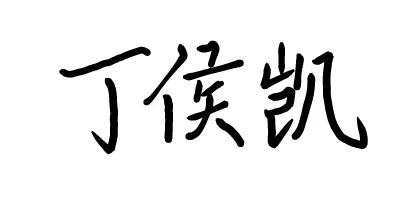
\includegraphics[width=2cm]{签名.jpg}
	& 评分: &\\
	\hline
	实验时间:&2024.9.27 & 教师签名:&\\
	\hline
	\end{tabularx}
\end{table}

\nsection{D2}{材料真空兼容测试和等离子特性研究}{实验记录}
\subsection{实验内容和步骤}
	\subsubsection{向真空中逐渐泵入空气恢复气压}
	\begin{enumerate}
		\item 给真空帕邢实验平台通电,打开真空计,观察真空时的气压大小。
		\item 打开通气阀并缓慢调节,产生进气声时停止调节,观察真空计的示数变化。
		\item 当内外气压相差不大时,均为$1.0*10^5Pa$时,即可打开放电腔体,观察内部结构。
	\end{enumerate}

	\subsubsection{使用机械泵与分子泵获得高真空环境}
	\begin{enumerate}
		\item 给真空帕邢实验平台通电,检查放电管与电源之间的电路连接是否可靠。
		\item 将电压调节旋钮调至最小位置;气体流量调节旋钮调至最小位置。
		\item 检查高压电源开关,分子泵电源开关是否处于断开状态。
		\item 插上机械泵、分子泵、帕邢高压电源插头,检查帕邢实验高压电源与放电腔𝐵𝑁𝐶接头连接是否正常。 
		\item 检查完毕后,推上空气开关,打开电源总开关。电源按钮、电源指示灯正常(呈现绿色)。 
		\item 记录初始气压为$1.0*10^5Pa$,开启机械泵,抽真空至2-3Pa,大约需要10分钟。
		\item 当放电腔内气压至$2-3Pa$时,按下分子泵电源,启动分子泵抽取放电腔内气压,此时分子泵转速会从 450 转降至 68 转左右进行自检,自检后开始从 68 转上升至 450 转。
		\item 抽取放电腔内气压为$1.5\times10^-3$时,调节气体流量控制旋钮至最小位置,调节电压到最小值,断开帕
		邢高压电源开关:先点击分子泵控制面板上的红色按钮,分子泵转速开始下降,需待转速降为零后断开分子泵电源开关,之后断开机械泵开关,电源总开关,推下空气开关,顺序切勿颠倒,否则将损坏分子泵。
		\item 记录抽取真空时的气压随时间变化数据,整理如\cref{tab:抽取真空过程中真空度随时间变化的数据记录}。
	\end{enumerate}

	% \usepackage{tabularray}
% \usepackage{tabularray}
\begin{table}
	\centering
	\begin{tblr}{
	  vline{3,5} = {-}{},
	  hline{1-2} = {-}{},
	}
	时间(S) & 气压大小 & 时间(S) & 气压大小   & 时间(S) & 气压大小   \\
	26    & 81   & 400   & 0,72   & 840   & 0,0035 \\
	36    & 20   & 420   & 0,2    & 860   & 0,0034 \\
	46    & 14   & 440   & 0,069  & 880   & 0,0033 \\
	56    & 11   & 460   & 0,038  & 900   & 0,0032 \\
	66    & 9,8  & 480   & 0,033  & 920   & 0,0031 \\
	76    & 8,8  & 500   & 0,026  & 940   & 0,0031 \\
	85    & 7,8  & 520   & 0,021  & 960   & 0,003  \\
	100   & 6,9  & 540   & 0,016  & 980   & 0,0029 \\
	120   & 6    & 560   & 0,012  & 1000  & 0,0028 \\
	140   & 5,3  & 580   & 0,0098 & 1020  & 0,0027 \\
	160   & 4,8  & 600   & 0,0082 & 1040  & 0,0026 \\
	180   & 4,4  & 620   & 0,0069 & 1060  & 0,0026 \\
	200   & 4    & 640   & 0,0061 & 1080  & 0,0025 \\
	220   & 3,7  & 660   & 0,0049 & 1100  & 0,0023 \\
	240   & 3,5  & 680   & 0,0047 & 1120  & 0,0023 \\
	260   & 3,3  & 700   & 0,0044 & 1140  & 0,0022 \\
	280   & 3,1  & 720   & 0,0044 & 1160  & 0,0022 \\
	300   & 2,9  & 740   & 0,0042 & 1180  & 0,0022 \\
	320   & 2,8  & 760   & 0,0041 & 1200  & 0,0022 \\
	340   & 2,6  & 780   & 0,0039 & 1220  & 0,0022 \\
	360   & 2,5  & 800   & 0,0038 &       &        \\
	380   & 2,4  & 820   & 0,0037 &       &        
	\end{tblr}
	\caption{抽取真空过程中真空度随时间变化的数据记录}
	\label{tab:抽取真空过程中真空度随时间变化的数据记录}
	\end{table}

	\begin{figure}[htbp]
			\centering
			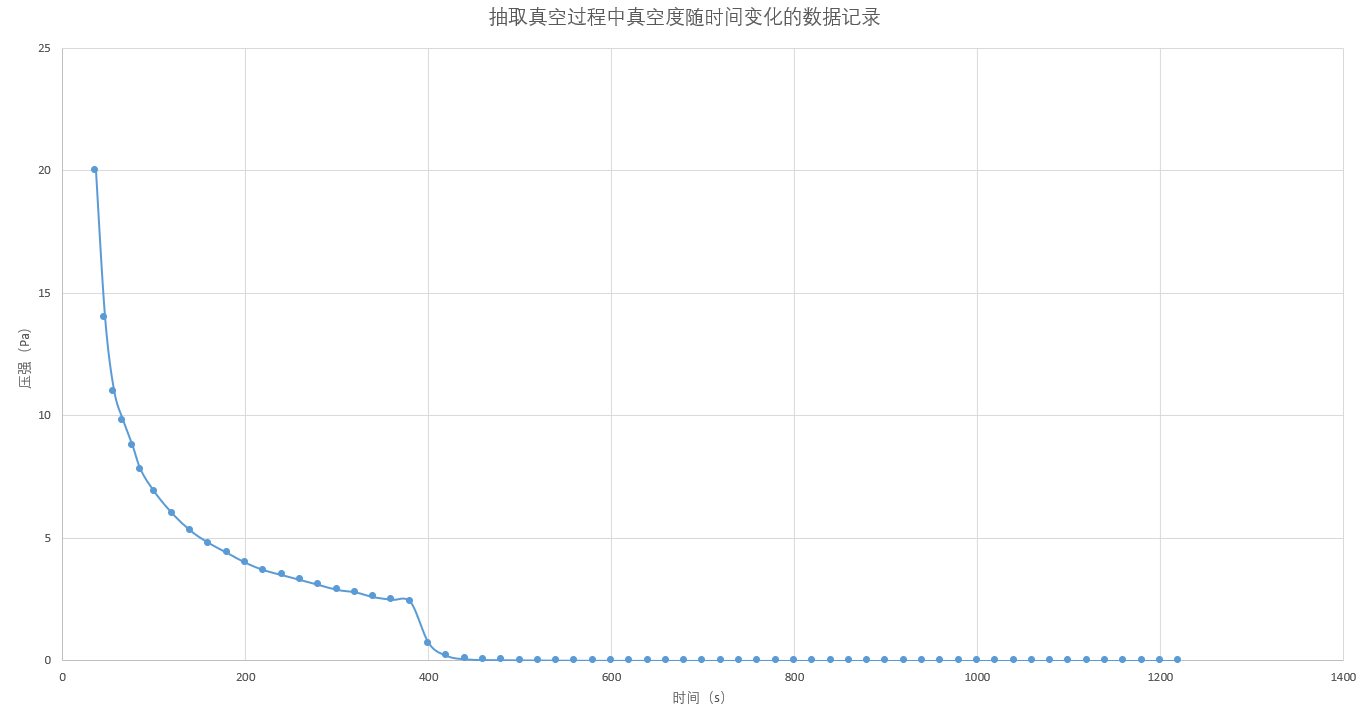
\includegraphics[width=0.75\textwidth]{真空图像.png}
			\caption{抽取真空过程中真空度随时间变化的数据记录}
			\label{fig:抽取真空过程中真空度随时间变化的数据记录}
	\end{figure}


	\subsubsection{验证帕邢定律}
	\begin{enumerate}
		\item 测量两电极之间的实际间距。
		\item 打开高压电源开关。
		\item 一名同学在旁边录像,另一名同学调节电源的电压输出,调节电源的电压输出快速增至 200V,然后继续缓慢升高电压,直
		至气体发生击穿现象。在视频中慢速观察击穿瞬间,读取击穿时的电压。记录气压和电压的数值。然后,把电压降至0V以下,为下一次测量做好准备。
		\item 在减小电压的过程中注意观察放电熄灭电压,并注意其与击穿电压的差别。
	\end{enumerate}
	\textcolor{red}{注意}:
\begin{enumerate}
	\item 增加电压过程中,应密切观察放电管电压表头和击穿电压表头的示数,避免电压过大超过量程导致表头损坏。
	\item 每个气压下可多次重复测量,取击穿电压测量值之间的偏差较小的数据为实验数据,以得到可靠击穿电压。
	\item 在气压较高时,击穿前后放电管的电压会有明显下降。应记录的电压为,击穿瞬间前的放电管电压为气体击穿电压。
	\item 依次增加气体流量,每次增加10Pa左右,重复击穿电压的测量。直至气压达到100Pa。
	\item 减小气压回复至20Pa左右,重复击穿电压的测量。 
	\item 依次减小气压,每隔2Pa测量一组数据,直至4Pa。测得7-8组数据即可。
	\item 实验完毕后,调节气体流量控制旋钮至最小位置,调节电压至最小值,依次关闭电压、机械泵、电源开关。 
\end{enumerate}
实验数据记录如下:

	\begin{table}[H]
		\centering
		\begin{tabular}{|c|c|c|c|c|}
			\hline
			气压/Pa & \multicolumn{3}{c|}{击穿电压/V} & 击穿电压平均值/V \\
			\hline
			100 & 795 & 796 & 801 & 797.3 \\
			\hline
			90 & 774 & 772 & 775 & 773.7 \\
			\hline
			80 & 741 & 743 & 738 & 740.7 \\
			\hline
			70 & 706 & 711 & 711 & 709.3 \\
			\hline
			60 & 669 & 660 & 676 & 668.3 \\
			\hline
			50 & 636 & 627 & 637 & 633.3 \\
			\hline
			40 & 580 & 573 & 567 & 573.3 \\
			\hline
			30 & 540 & 536 & 529 & 535 \\
			\hline
			20 & 474 & 477 & 481 & 477.3 \\
			\hline
			18 & 476 & 474 & 456 & 468.7 \\
			\hline
			16 & 475 & 467 & 456 & 466 \\
			\hline
			14 & 459 & 450 & 437 & 448.7 \\
			\hline
			12 & 474 & 472 & 478 & 474.7 \\
			\hline
			10 & 500 & 498 & 476 & 491.3 \\
			\hline
			8 & 554 & 532 & 532 & 539.3 \\
			\hline
			6 & 650 &  642 & 656 & 649.3 \\
			\hline
			4 & 964 & 843 & 875 & 894 \\
 			\hline
		\end{tabular}
		\caption{气体放电实验数据(极板间距=4.80cm)}
		\label{tab:气体放电实验数据(极板间距=4.80cm)}
	\end{table}		

\subsubsection{观察气体发光现象}
\begin{enumerate}
	\item 打开光谱分析软件,设置积分时间为500ms,平均次数为10,触发模式为normal。
	\item 将光谱仪的感光元件放置在靠近真空腔,正对着气体电离发光区域,点击reference按钮存储背景光谱,记录背景光谱如\cref{fig:背景光谱}。
	\item 依次开启电源开关,机械泵和高压电源,调节气体流量控制旋钮,使真空腔内空气气压为 10𝑃𝑎,此时调节电源的电压输出气体发生击穿现象,存储下此时的等离子体光谱,并记录此时的击穿电流,记录的空气等离子体光谱如\cref{fig:空气等离子体光谱}。然后,把电压降至 0V 以下,为下一次测量做好准备。 实验数据记录如\cref{tab:等离子体光谱实验数据}。
	\item 得到光谱后旋紧空气的输入阀门,停止输入空气,打开氩气输入阀门,调节气体流量控制旋钮,使真空腔内气压达到稳定,输入氩气较长时间后,绝大部分空气被排出,此时真空腔内气压为3.8Pa,重复(2)中操作得到氩气电离的等离子体光谱。氩气中的等离子体发光为暗红色,记录氩气等离子体光谱如\cref{fig:氩气等离子体光谱}。
	\item 重复(3)中操作,依次得到氖气和氦气的等离子体光谱。发现氖气的等离子体发砖红色光,氦气发红色光(较亮),记录氖气等离子体光谱如\cref{fig:氖气等离子体光谱},记录氦气等离子体光谱如\cref{fig:氦气等离子体光谱}。
	\item 实验完毕后,调节气体流量控制旋钮至最小位置,调节电压至最小值,依次关闭电压、机械泵、电源开关。
\end{enumerate}

	\begin{figure}[htbp]
		\centering
		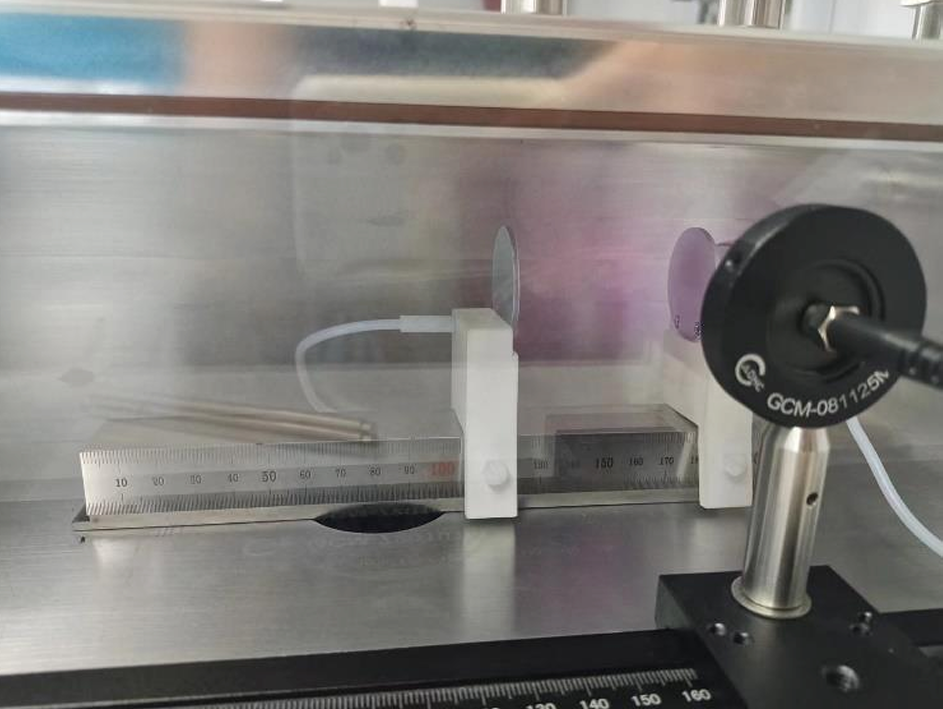
\includegraphics[width=0.45\textwidth]{实验观察记录.png}
		\caption{实验观察记录}
		\label{fig:实验观察记录}
	\end{figure}

	\begin{figure}[htbp]
		\centering
		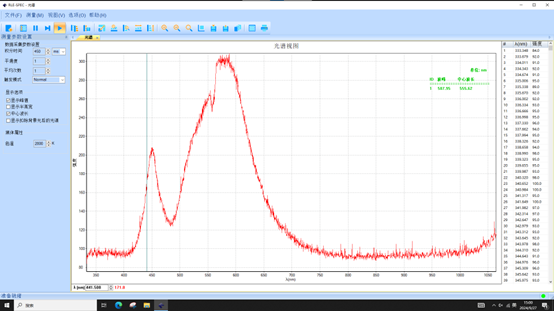
\includegraphics[width=0.90\textwidth]{背景光谱.png}
		\caption{背景光谱}
		\label{fig:背景光谱}
	\end{figure}

	\begin{figure}[htbp]
		\centering
		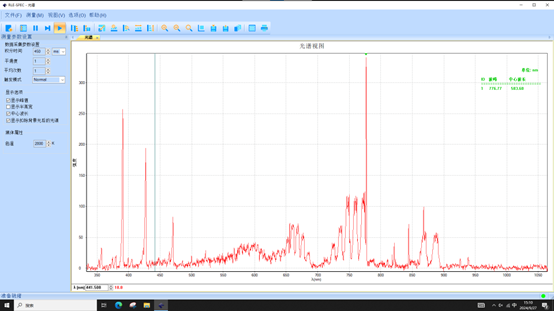
\includegraphics[width=0.90\textwidth]{空气等离子体光谱.png}
		\caption{空气等离子体光谱,气压12pa,击穿电压446v,击穿电流600$uA$}
		\label{fig:空气等离子体光谱}
	\end{figure}

	\begin{figure}[htbp]
		\centering
		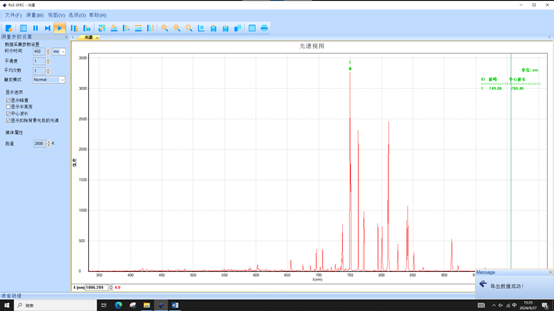
\includegraphics[width=0.90\textwidth]{氩气等离子体光谱.png}
		\caption{氩气等离子体光谱,气压24pa,击穿电压328v}
		\label{fig:氩气等离子体光谱}
	\end{figure}
	
	\begin{figure}[htbp]
		\centering
		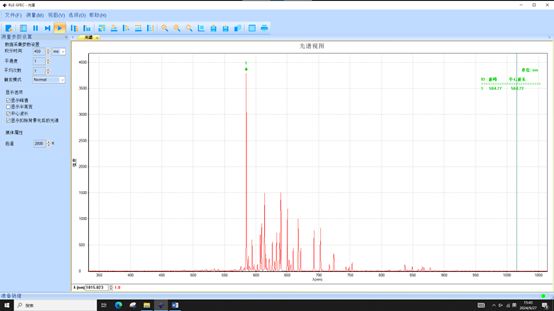
\includegraphics[width=0.90\textwidth]{氖气等离子体光谱.png}
		\caption{氖气等离子体光谱,气压24pa,击穿电压436v,击穿电流600$uA$}
		\label{fig:氩气等离子体光谱}
	\end{figure}

	\begin{figure}[htbp]
		\centering
		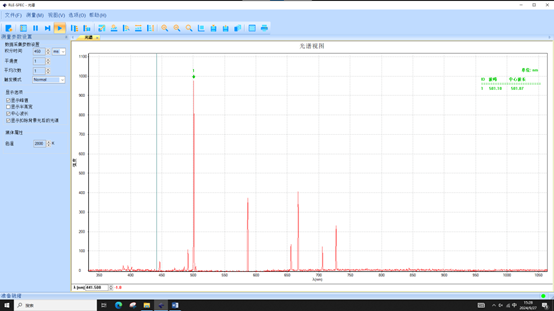
\includegraphics[width=0.90\textwidth]{氦气等离子体光谱.png}
		\caption{氦气等离子体光谱,气压24pa,击穿电压725V}
		\label{fig:氦气等离子体光谱}
	\end{figure}
	

	\begin{table}[!ht]
		\centering
		\begin{tabular}{|l|l|l|l|}
		\hline
			气压/Pa & 气体 & 电压/V & 电流/uA \\ \hline
			12 & 空气 & 446 & 600 \\ \hline
			24 & 氦气 & 725 & 600 \\ \hline
			24 & 氖气 & 436 & 600 \\ \hline
			24 & 氩气 & 328 & 600 \\ \hline
		\end{tabular}
		\caption{等离子体光谱实验数据}
		\label{等离子体光谱实验数据}
	\end{table}

	\subsubsection{运用四极质谱仪以及 VAccuRay3.0 软件进行实验}
	\begin{enumerate}
		\item 重复实验1中抽真空操作,观察真空计显示屏,待分子泵抽取至真空腔内气压为 5.0×10−2𝑃𝑎 以下后打开四极质谱仪。
		\item 打开测试软件 VAccuRay3.0 进行实验。 
		\item 打开软件后点击右键,选择 Device setup, Device setup, 出现以下界面:
		\begin{figure}[htbp]
			\centering
			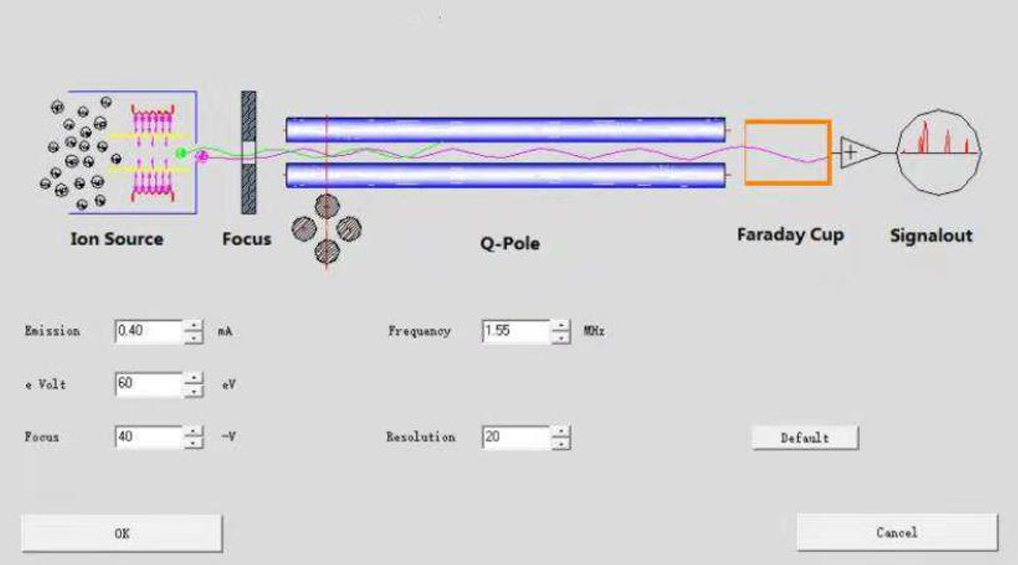
\includegraphics[width=0.90\textwidth]{四极质谱仪软件参数.png}
			\caption{四极质谱仪软件参数}
			\label{fig:四极质谱仪软件参数}
		\end{figure}
		\item 然后点击任务栏灯丝选项,此时会出现“Be Sure pressure Less Than 5.0E-2pa.”提示,观察真空计确定真空度低于该提示值是才
		能点击确定,否则将损坏四极质谱仪的灯丝,发生危险。 
		\item 点击确认后会出现 Spectrum 质谱图,此时即可通过各种粒子的相对分质量确定气体的波峰。通过软
		件得到本底的质谱图。
		\begin{figure}[htbp]
			\centering
			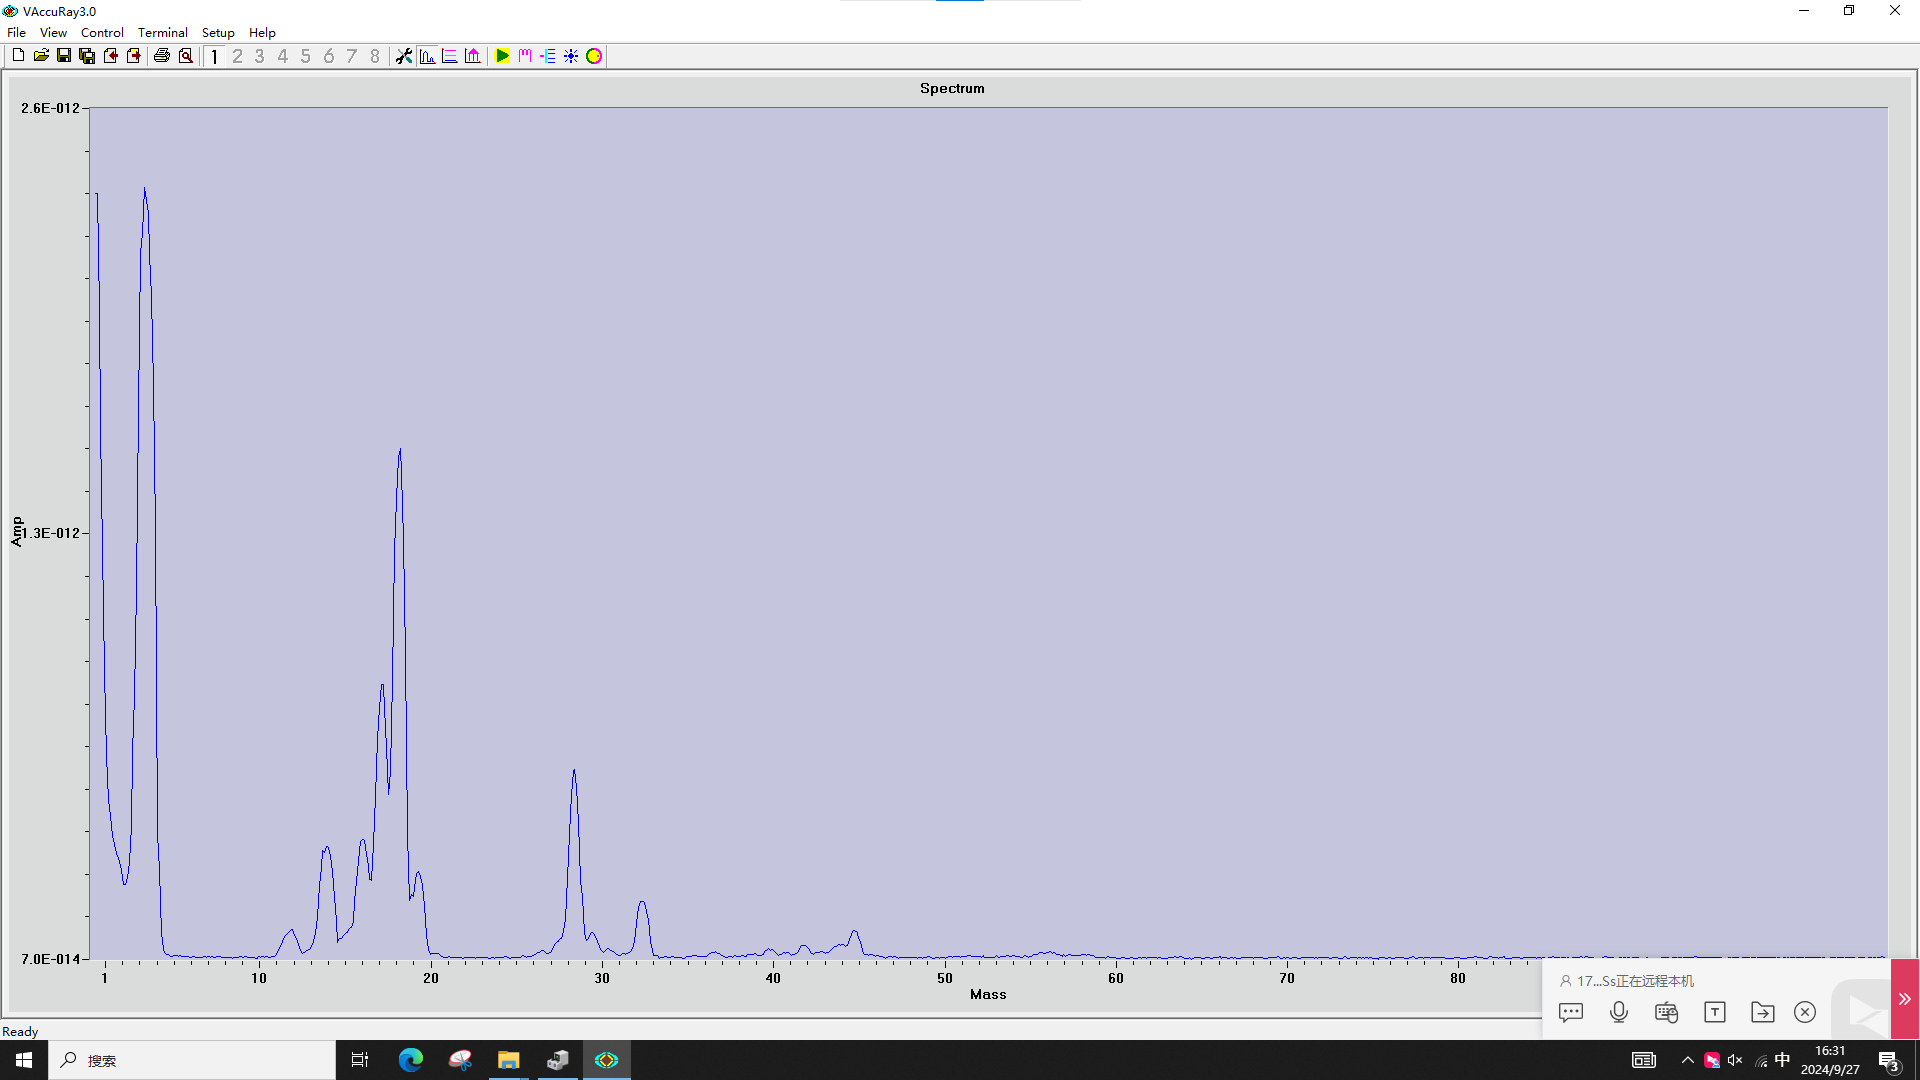
\includegraphics[width=0.90\textwidth]{本底质谱图.png}
			\caption{本底质谱图,压强为7.8E-4Pa}
			\label{fig:本底质谱图}
		\end{figure}
		\item 点击 OK 后,重复(3)(4)(5)(6)(7)步骤,依次通入空气、𝐻𝑒、𝐴𝑟、𝑁𝑒 气,并记录数
		据。测得质谱前,我们需要长时间通入待测气体以排除绝大部分杂质气体,得到更纯净的气体质谱。 
		\item 实验结束后,先按分子泵电源面板处红色按钮,待转速降为 0 时,才能断开分子泵电源开关,断开
		分子泵电源开关后才能断开机械泵开关,顺序切勿颠倒,否则将损坏分子泵,最后关闭总电源。 
		\item 整理数据,进行总结,实验数据整理如下:
		\begin{figure}[htbp]
			\centering
			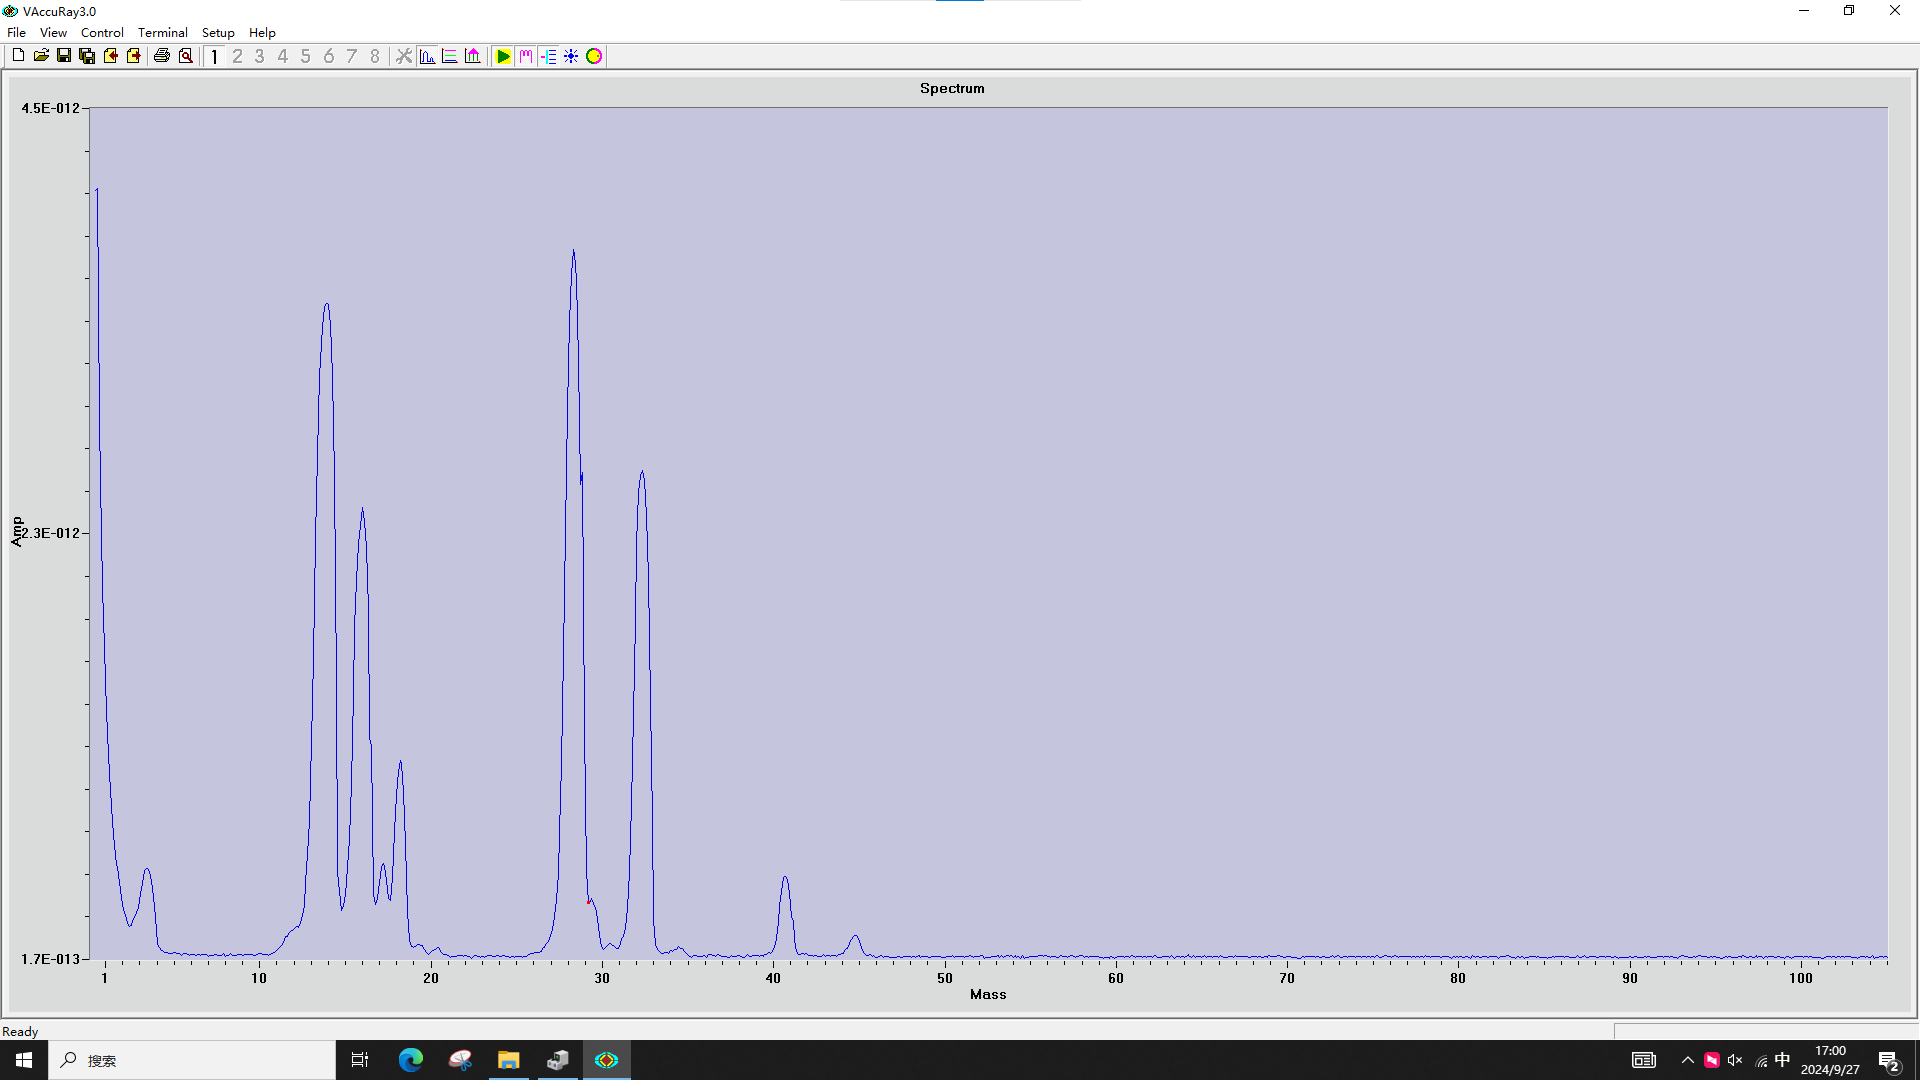
\includegraphics[width=0.90\textwidth]{空气质谱图.png}
			\caption{空气质谱图,压强为0.025Pa}
			\label{fig:空气质谱图}
		\end{figure}
		
		\begin{figure}[htbp]
			\centering
			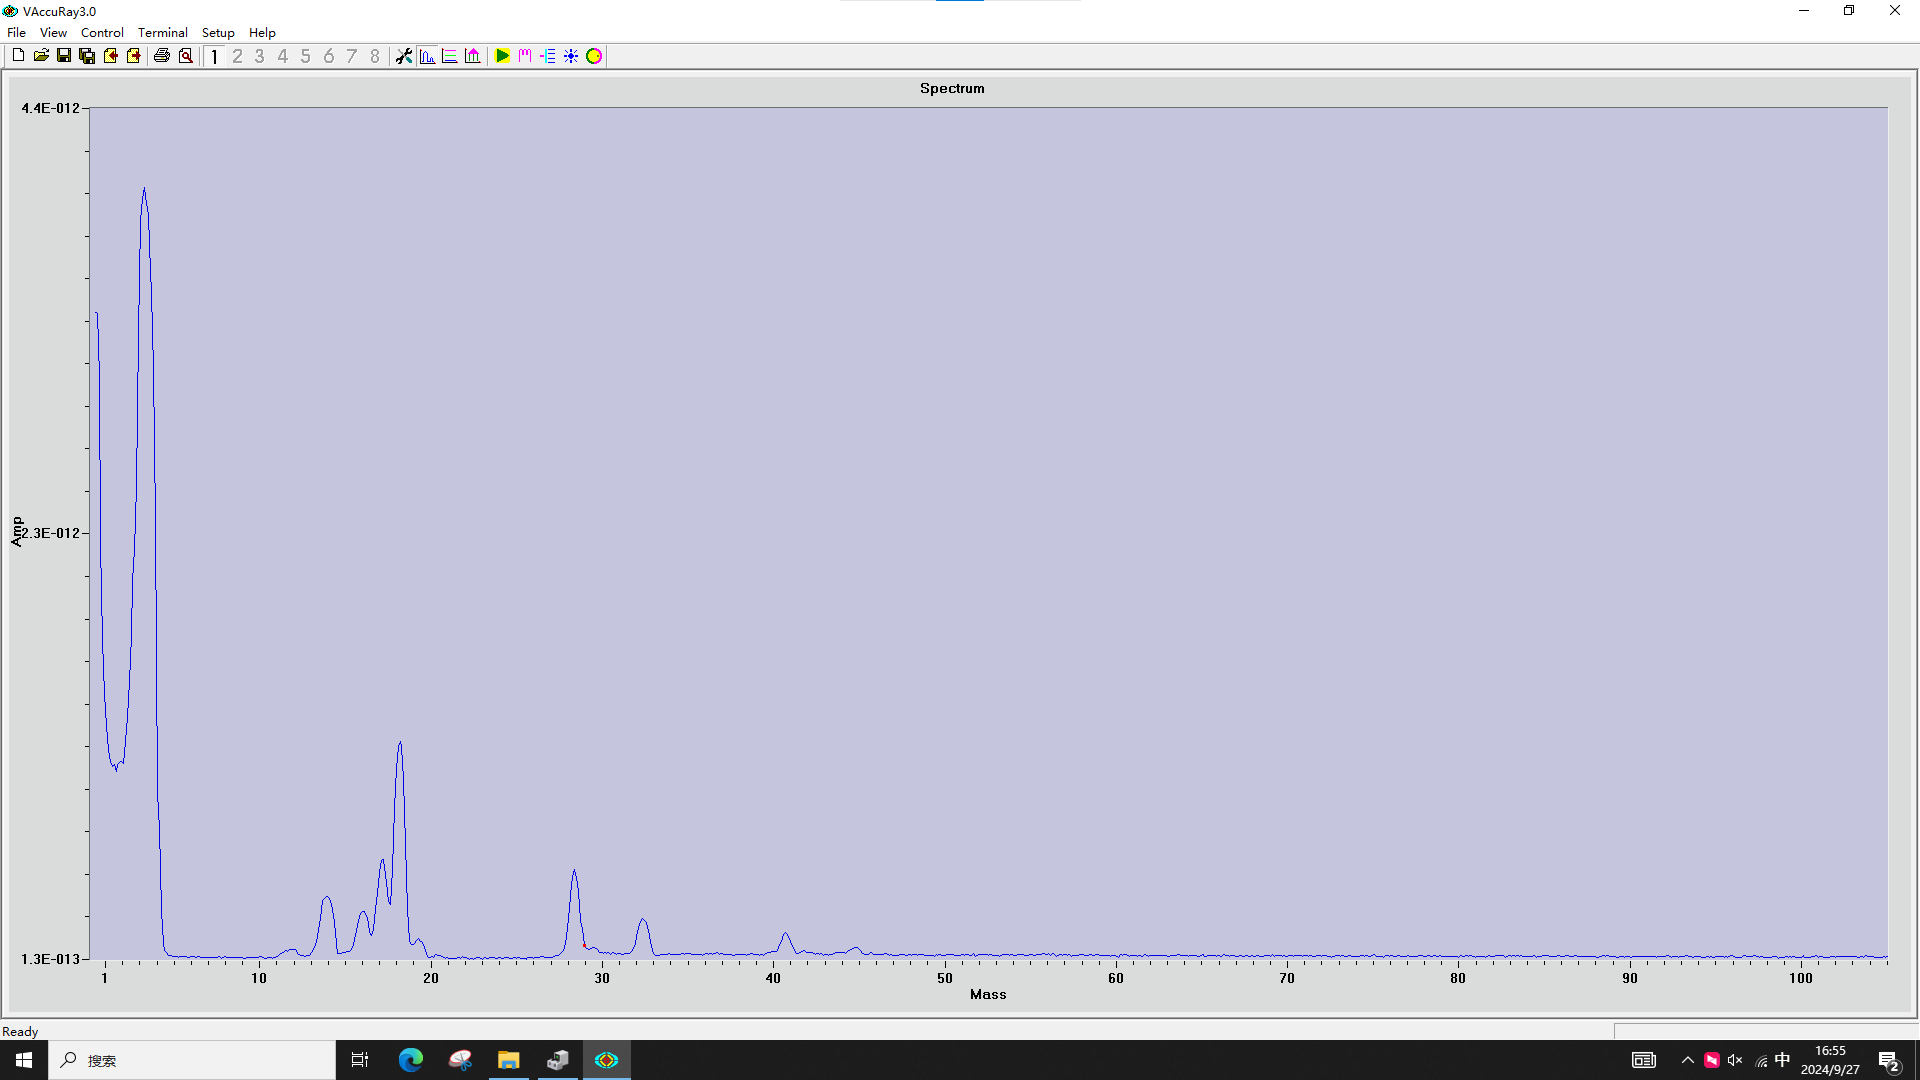
\includegraphics[width=0.90\textwidth]{氦气质谱图.png}
			\caption{氦气质谱图,压强为0.003Pa}
			\label{fig:氦气质谱图}
		\end{figure}

		\begin{figure}[htbp]
			\centering
			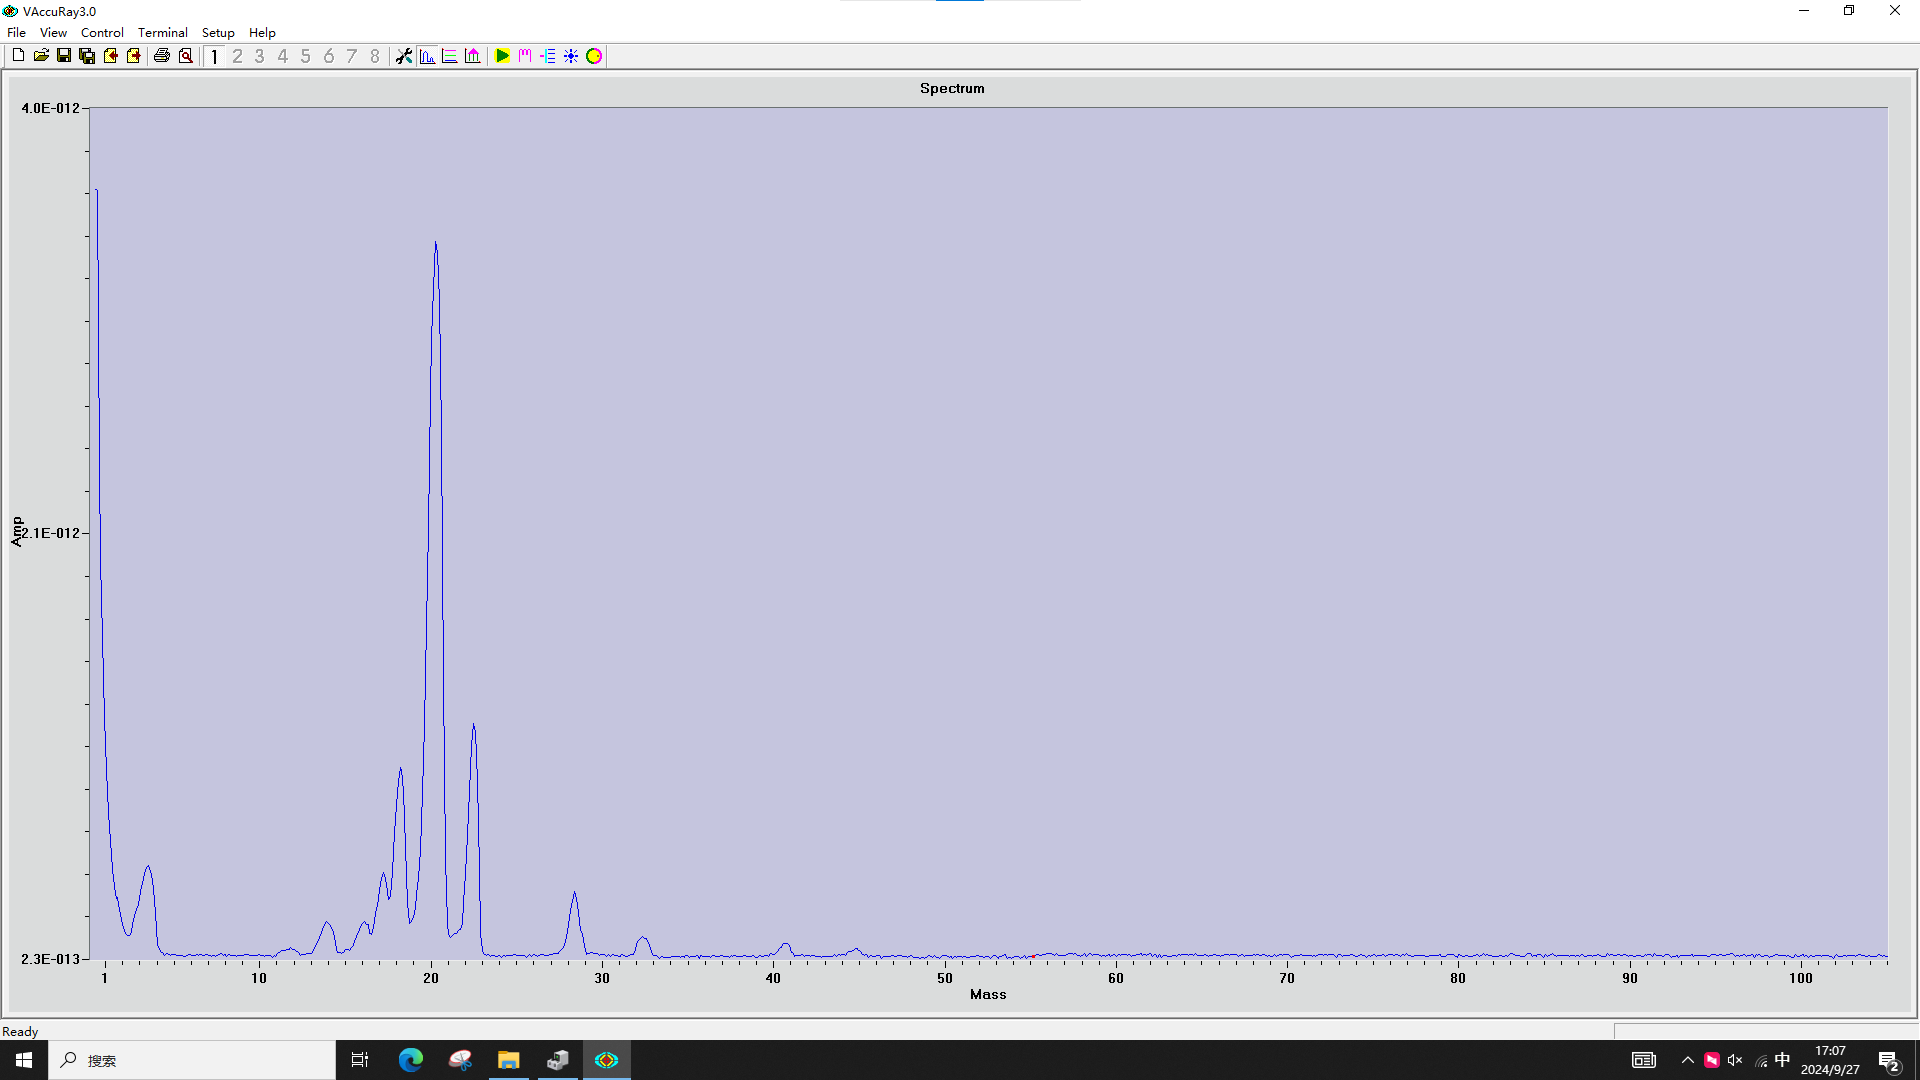
\includegraphics[width=0.90\textwidth]{氖气质谱图.png}
			\caption{氖气质谱图,压强为0.016Pa}
			\label{fig:氖气质谱图}
		\end{figure}
		
		\begin{figure}[htbp]
			\centering
			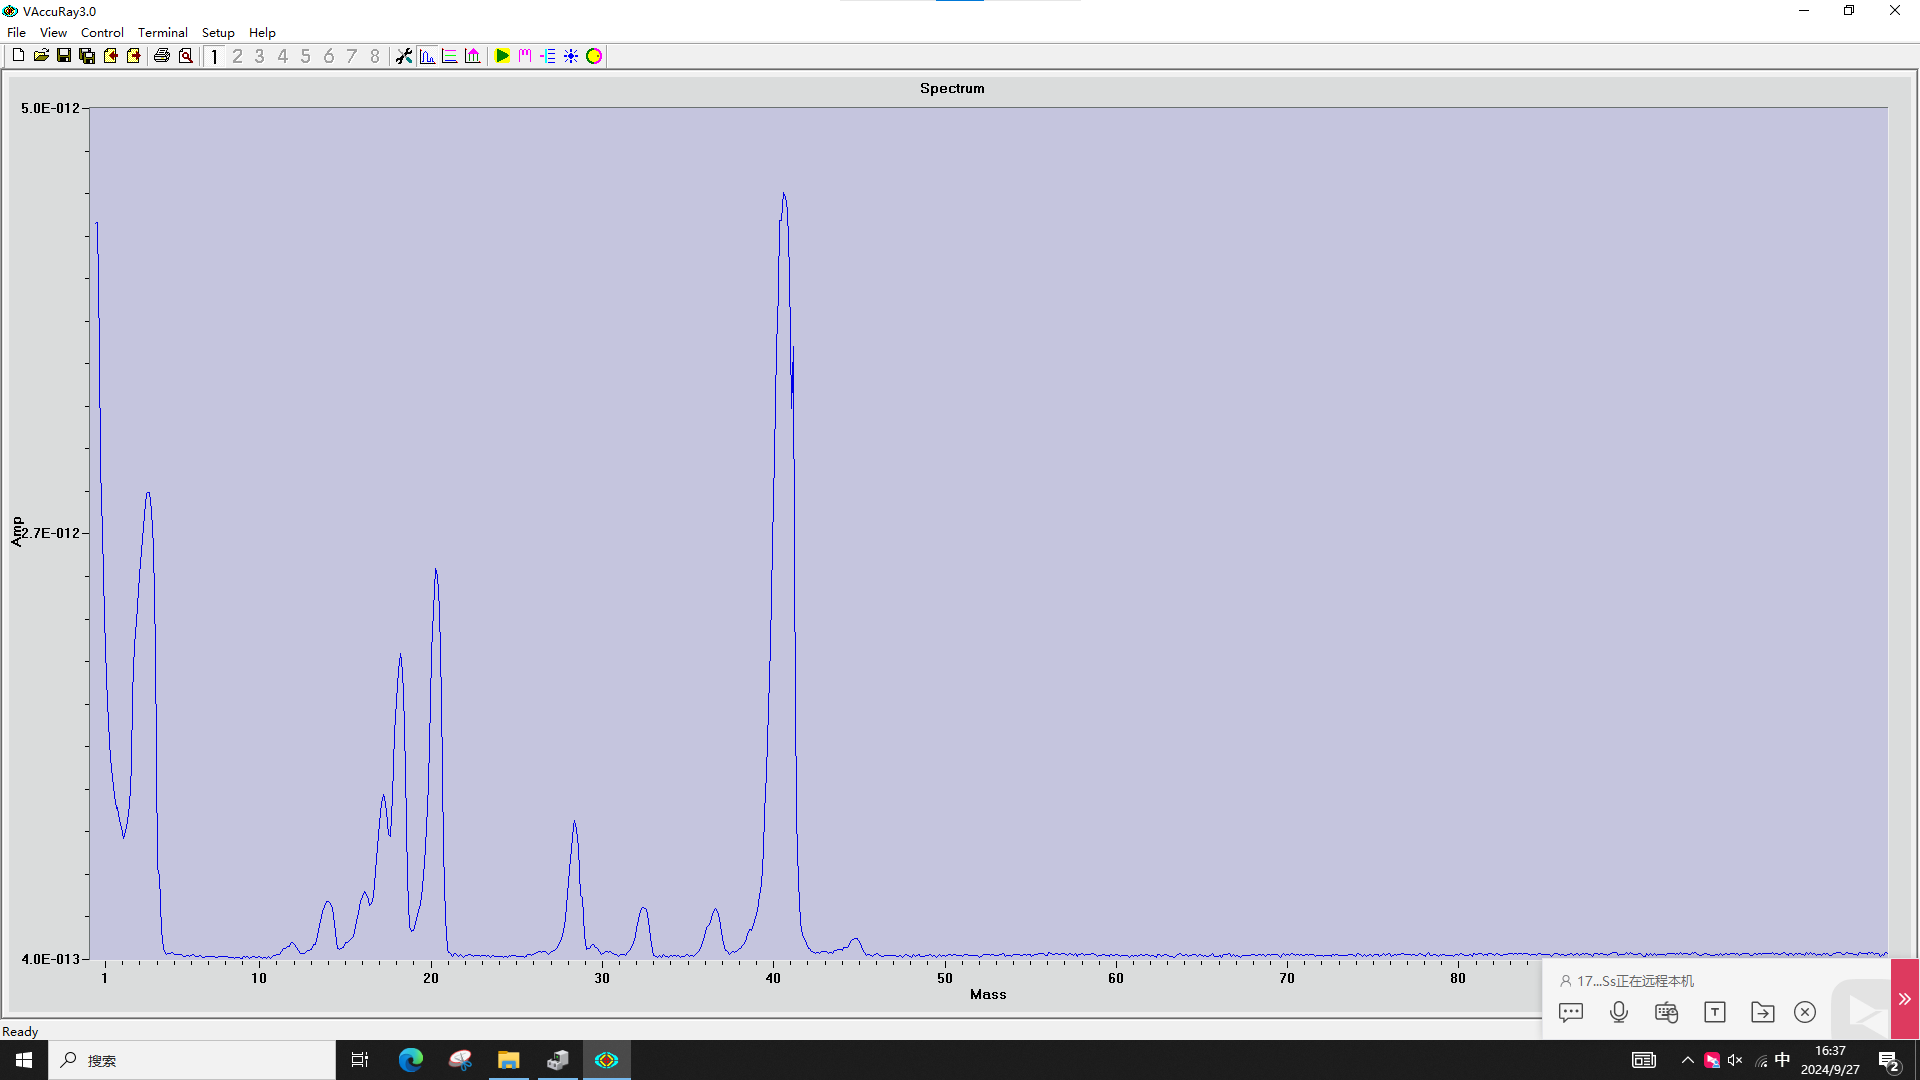
\includegraphics[width=0.90\textwidth]{氩气质谱图.png}
			\caption{氩气质谱图,压强为0.032Pa}
			\label{fig:氩气质谱图}
		\end{figure}
	\end{enumerate}

\clearpage

\subsection{原始数据记录}
\begin{figure}[htbp]
	\centering
	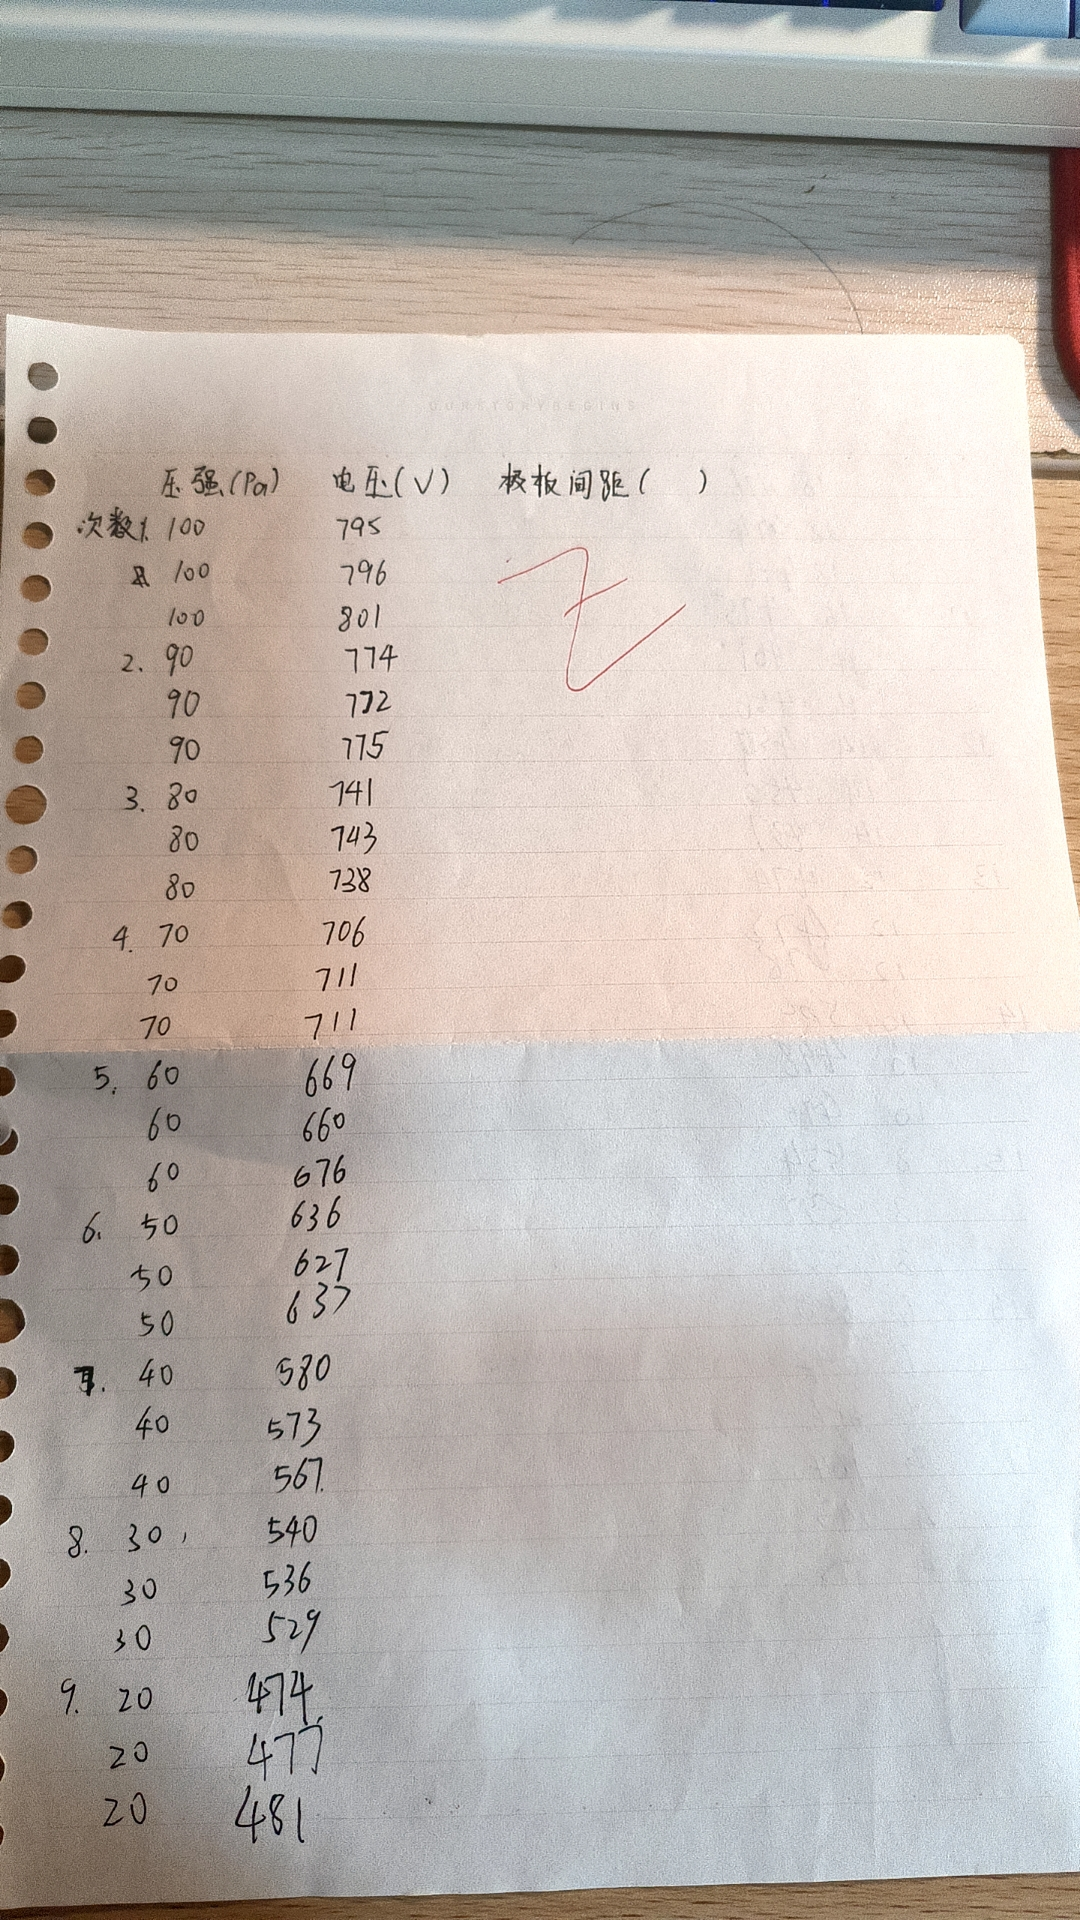
\includegraphics[width=0.45\textwidth]{原始数据记录.jpg}
	\caption{原始数据记录}
	\label{fig:原始数据记录}
\end{figure}

\begin{figure}[htbp]
	\centering
	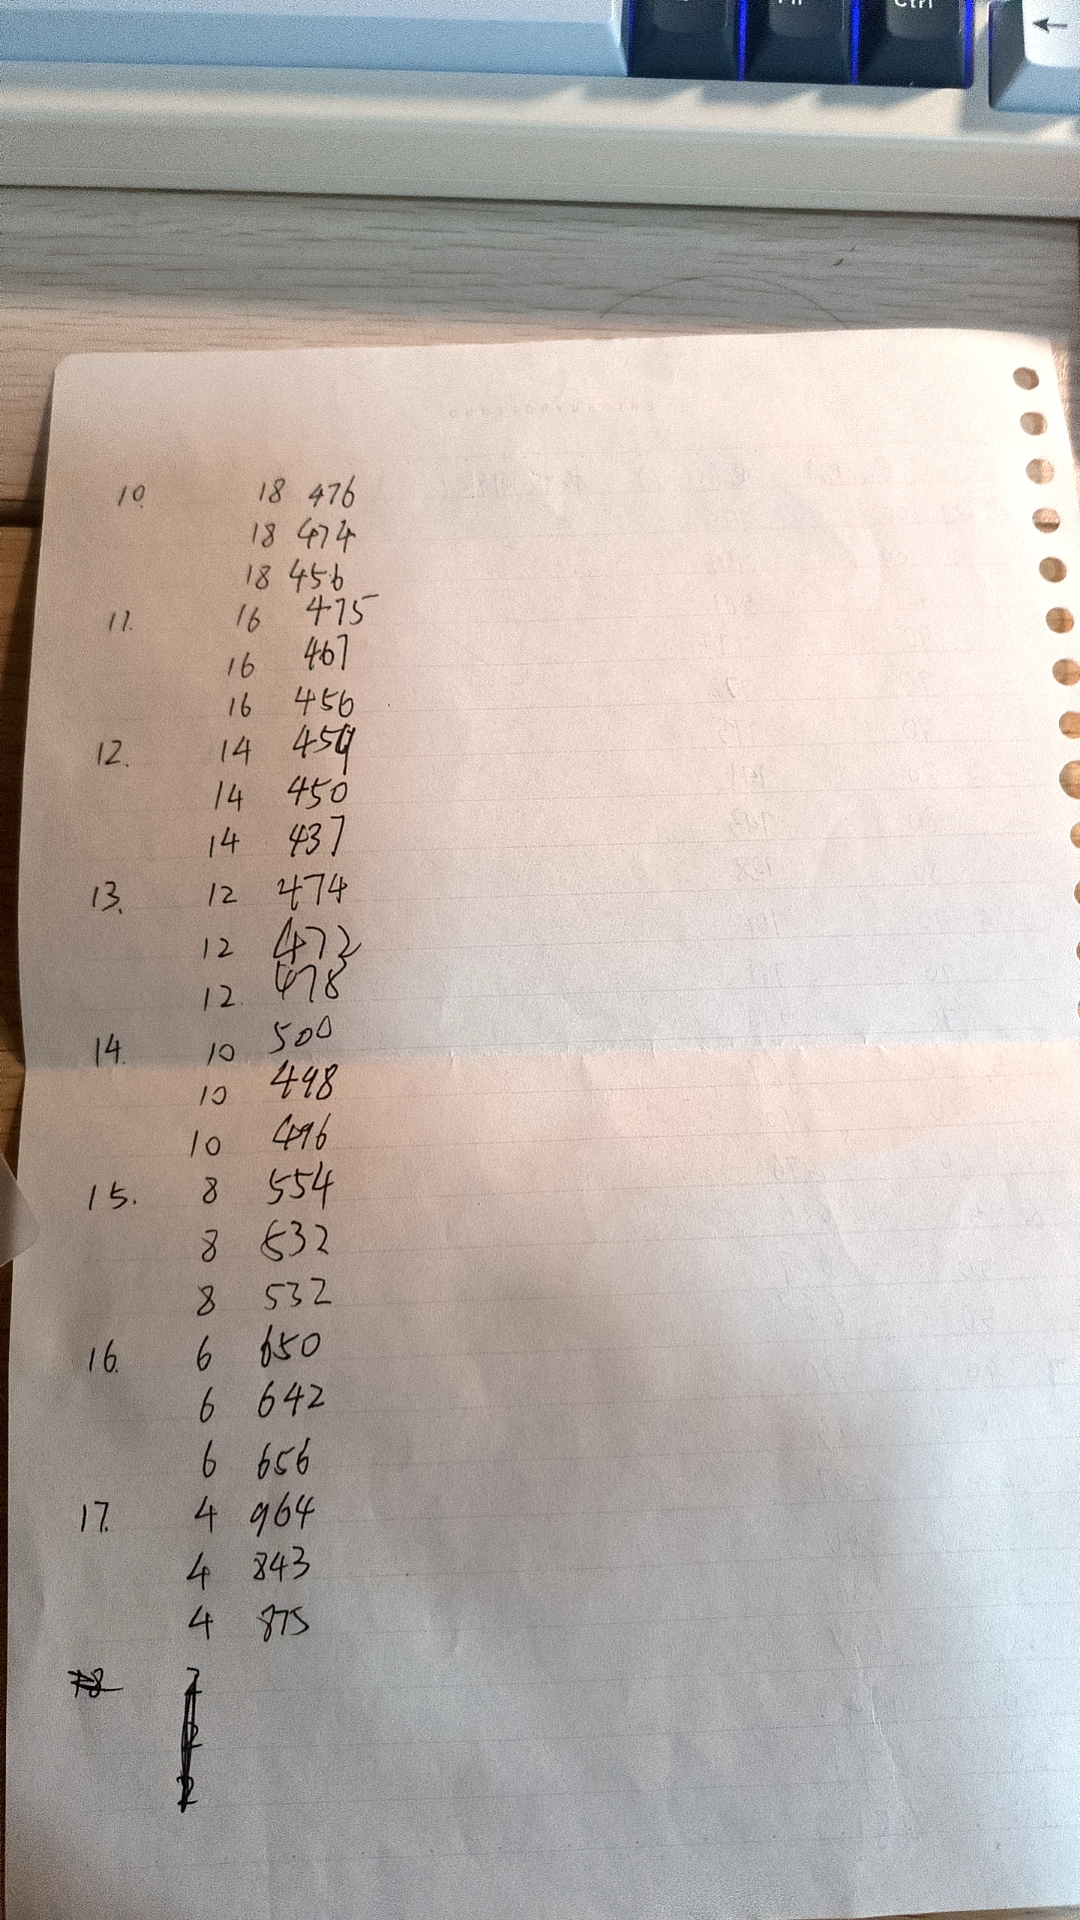
\includegraphics[width=0.45\textwidth]{原始数据记录2.jpg}
	\caption{原始数据记录}
	\label{fig:原始数据记录2}
\end{figure}

\clearpage
\subsection{实验过程中遇到的问题记录}
	\begin{enumerate}
		\item 由于初始参数不正确,导致四级质谱仪一开始未能正常工作。调整完初始参数之后四级质谱仪工作正常。
	\end{enumerate}






\clearpage
\begin{table}
	\renewcommand\arraystretch{1.7}
	\begin{tabularx}{\textwidth}{|X|X|X|X|}
	\hline
	专业:& 物理学 &年级:& 2022级\\
	\hline
	姓名: &丁侯凯 & 学号:&22344009 \\
	\hline
    日期:& 2024.9.27& 评分: &\\
	\hline
	\end{tabularx}
\end{table}

\nsection{D2}{材料真空兼容测试和等离子特性研究}{分析与讨论}
\subsection{实验数据分析}
	\subsubsection{使用机械泵与分子泵获取高真空时,真空度随时间变化的曲线}
	\begin{figure}[htbp]
		\centering
		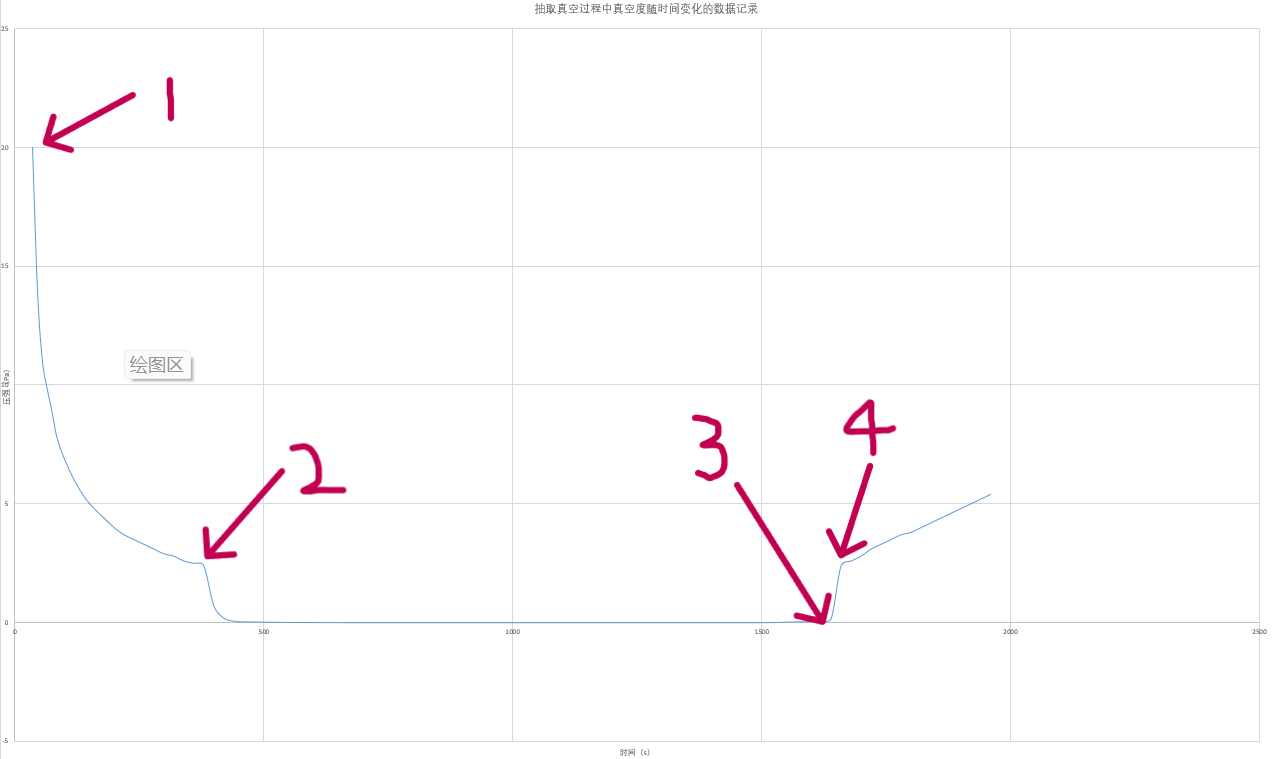
\includegraphics[width=0.90\textwidth]{真空度随时间变化图像.png}
		\caption{真空度随时间变化图像}
		\label{fig:真空度随时间变化图像}
	\end{figure}
	其中:
	\begin{enumerate}
		\item 时刻1:开启机械泵。
		\item 时刻2:开启分子泵。
		\item 时刻3:分子泵转速为零。
		\item 时刻4:关闭机械泵。
	\end{enumerate}

	\subsubsection{测量击穿电压与电极间隙和气压之间的关系,验证帕邢定律}
	已知帕邢定律的公式为:
	\begin{equation}
	V_s = \frac{BPd}{\ln(\frac{APd}{\ln(1+Y)})}
	\label{eq:帕邢定律公式}
	\end{equation}
	取平均值得到d=0.048m。
	
	\begin{figure}[htbp]
		\centering
		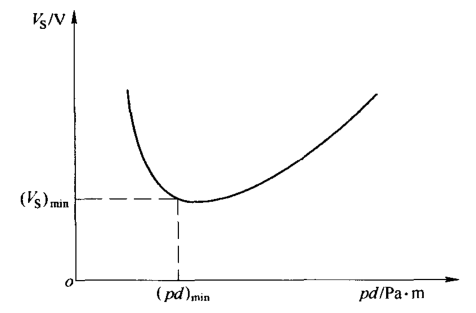
\includegraphics[width=0.55\textwidth]{帕邢定律.png}
		\caption{帕邢定律}
		\label{fig:帕邢定律}
	\end{figure}
	气压大小与击穿电压大小数据如\cref{tab:气体放电实验数据(极板间距=4.80cm)},绘制帕邢定律图像如下:
	\begin{figure}[htbp]
		\centering
		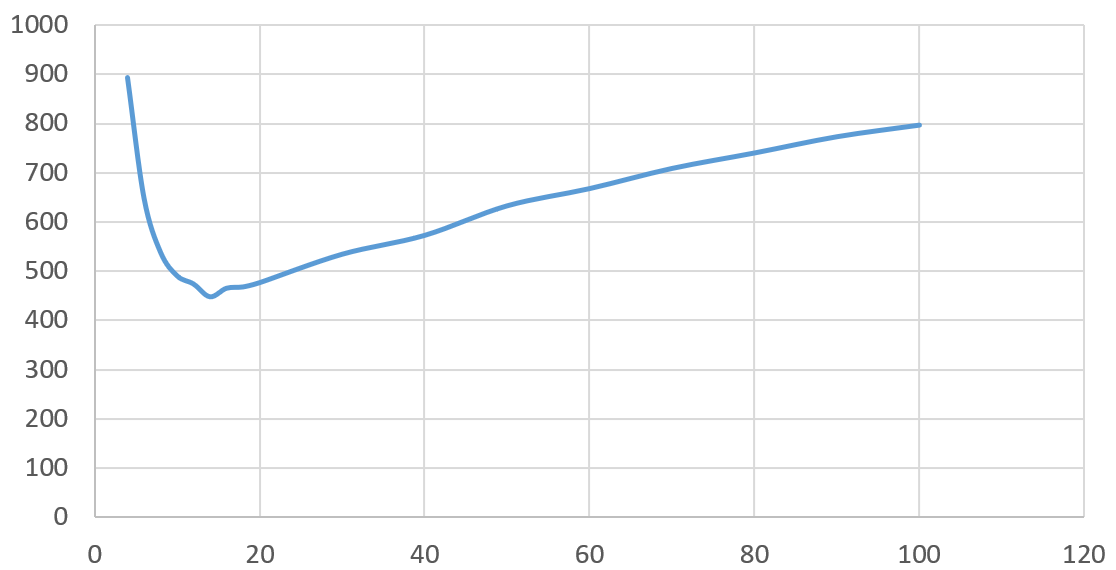
\includegraphics[width=0.55\textwidth]{帕邢定律实验数据.png}
		\caption{帕邢定律实验数据}
		\label{fig:帕邢定律实验数据}
	\end{figure}
	与标准大气压情况下帕邢定律曲线相比较:实验测得的帕邢定律曲线与理论较为吻合,因此可以验证帕邢定律。同时我们可以得到空气中,曲线在特定的 $Pd$=0.580$Pa*m$ 值时,有最小的击穿电压。 

	\subsubsection{研究气体放电产生的等离子体光谱特性 }
	实验所测数据如\cref{fig:背景光谱}、\cref{fig:空气等离子体光谱}、\cref{fig:氦气等离子体光谱}、\cref{fig:氩气等离子体光谱}所示:
	\begin{enumerate}
		\item 实验观察到空气帕邢放电发出紫光;实验几乎观察不到氩气帕邢放电的光;实验观察到氦气帕邢放电发出较弱的绿光;实验观察到氦气帕邢放电发出红橙光。
		\item 空气等离子体光谱第一波峰对应波长776.77nm对应O原子中电子从3p轨道跃迁到3s轨道的跃迁谱线;第二波峰对应波长为390.57nm对应O离子由3d轨道跃迁到3p轨道;第三波峰对应C原子中电子由3p跃迁到3s;半高宽取决于离子温度和密度,正比于离子密度,可以推断出上述三种跃迁的发生比例约为1:2:2。
		\item 氩气等离子体光谱第一波峰对应波长750.23nm对应Ar原子电子从4p轨道跃迁到4s轨道(1/2)的跃迁谱线,第二波峰对应波长为811.38nm对应Ar离子由4p轨道跃迁到3d轨道,第三波峰同样对应波长为763.37nm对应Ar离子由4p轨道跃迁到4s轨道,通过半高宽可以推断出上述三种跃迁的发生比例约为2:1:1。 
		\item 氖气等离子体光谱第一波峰对应波长584.73nm对应Ne原子电子从3p轨道跃迁到3s轨道的跃迁谱线,第二波峰对应波长为613.88nm对应Ne离子由4d轨道跃迁到3p轨道,第三波峰对应波长为763.37nm对应Ne原子由5s轨道跃迁到3p轨道,通过半高宽可以推断出上述三种跃迁的发生比例约为1:1:1。 
		\item 氖气等离子体光谱第一波峰对应波长501.11nm对应He原子电子从3p轨道跃迁到2s轨道的跃迁谱线,第二波峰对应波长为667.61nm对应Ne离子由3d轨道跃迁到2p轨道,第三波峰同样对应波长为587.21nm对应He原子由3d轨道跃迁到2p轨道,通过半高宽可以推断出上述三种跃迁的发生比例约为1:1:1。 
	\end{enumerate}


	
	\subsubsection{通过质谱分析气体种类及含量  }
	实验所测数据如\cref{fig:本底质谱图}、\cref{fig:氖气质谱图}、\cref{fig:氦气质谱图}、\cref{fig:氩气质谱图}所示:
	\begin{enumerate}
		
		\item 根据本底质谱,我们可以分析得到几个波峰对应的质量数分别为2(对应𝐻2)、18(对应𝐻2𝑂)。而根据半高
		宽与峰值高低,我们可以推断本底质谱中水蒸气占比最高。 
		\item 分析空气的质谱,几个波峰对应的质量数分别为2(对应𝐻2)、18(对应𝐻2𝑂)、28(对应𝑁2)、32(对应
		2)、40(对应𝐶𝑂2)。
		\item 分析氦气的质谱,几个波峰对应的质量数分别为2(对应𝐻2)、4(对应𝐻𝑒)、18(对应𝐻2𝑂),其中 𝐻𝑒含
		量最高,但仍存在部分𝐻2和𝐻2𝑂。
		\item 分析氩气的质谱,几个波峰对应的质量数分别为2(对应𝐻2)、18(对应𝐻2𝑂)、40(对应𝐴𝑟),其中 𝐴𝑟
		含量最高,但仍存在部分𝐻2和𝐻2𝑂,减去本底后𝐴𝑟占比更高。
		\item 分析氖气的质谱,几个波峰对应的质量数分别为2(对应𝐻2)、18(对应𝐻2𝑂)、20(对应𝑁𝑒),其中 𝑁𝑒
		含量最高,但仍存在部分𝐻2和𝐻2𝑂,减去本底后𝑁𝑒占比更高。
	\end{enumerate}

	\subsection{实验心得和体会}
	\begin{enumerate}
		\item 大致上我们的实验完成的比较成功,实验现象与结果都较能符合理论。但实验所需要的时间的确较长,由于对实验仪器的不熟悉,会导致前期工作延长。
		\item 在对于帕邢定律的数学拟合中,由于无法客观原因无法使用更精确的拟合软件,导致拟合得到的曲线精确度较低,并且无法将两个图像叠加起来算出帕邢定律的几个常数,之后可以改进。
		\item 感谢\textbf{周老师}在实验中的耐心指导与教诲,让我们能够顺利完成实验。
	\end{enumerate}
	\quad \large \textbf{感谢您对于此篇实验报告的阅读与批改,祝您工作顺利!}
\clearpage


% ---------------------------------------------------------------------
%   参考文献
%   注:使用参考文献时应按照xelatex->bibtex->xelatex->xelatex顺序进行编译
\phantomsection
\addcontentsline{toc}{section}{参考文献}
\bibliographystyle{unsrt}1. 巴德纯 等翻译,真空技术手册(TheVacuumTechnologyBook),普发真空(PfeifferVacuum),2013 年。

2. 华中一 主编,真空实验技术,上海科学技术出版社,1986年。

3. 胡汉泉,王迁 等主编,真空物理与技术及其在电子器件中的应用,国防工业出版
社,1982年。

4. 徐学基,诸定昌 编著,气体放电物理,复旦大学出版社,1996年。

5. 金佑民,樊友三 编著,低温等离子体物理基础,清华大学出版社,1983年。

6. 徐金瑞,田笠卿 编著,ICP发射光谱分析,南京大学出版社,1990年。

7. 李潮锐 等编,《物理学实验教程(近代物理实验)》,中山大学出版社,2004年。

8. 乐永康,复旦大学等离子体物理实验讲义。

9. 上海宜准电子科技有限公司,宜准VQP01真空机组和平台使用说明书、宜准四极质

谱仪使用说明书,2018年。

10. 维基百科。
\bibliography{myref}

% \clearpage
% \appendix
% \appendixpage
% \addappheadtotoc

% \begin{tbox}{字体设置(中文)}
% \begin{enumerate}
% 	\item 宋体:{\songti 山有扶苏,隰有荷华}
% 	\item 仿宋:{\fangsong 山有扶苏,隰有荷华}
% 	\item 黑体:{\heiti 山有扶苏,隰有荷华}
% 	\item 楷书:{\kaishu 山有扶苏,隰有荷华}
% \end{enumerate}
% \end{tbox}

% \begin{tbox}{Set font(English)}
% \begin{enumerate}
% 	\item roman:\quad{\rmfamily Hello world!}
% 	\item sans-serif:\quad{\sffamily Hello world!}
% 	\item typewriter:\quad{\ttfamily Hello world!}
% \end{enumerate}
% \end{tbox}

% \begin{tbox}{公式}
% 	无编号公式
%     \begin{equation*}
%         J(\theta) = \mathbb{E}_{\pi_\theta}[G_t] = \sum_{s\in\mathcal{S}} d^\pi (s)V^\pi(s)=\sum_{s\in\mathcal{S}} d^\pi(s)\sum_{a\in\mathcal{A}}\pi_\theta(a|s)Q^\pi(s,a)
%     \end{equation*}
% $$ J(\theta) = \mathbb{E}_{\pi_\theta}[G_t] = \sum_{s\in\mathcal{S}} d^\pi (s)V^\pi(s)=\sum_{s\in\mathcal{S}} d^\pi(s)\sum_{a\in\mathcal{A}}\pi_\theta(a|s)Q^\pi(s,a) $$
%     有编号公式
%     \begin{equation}
%         J(\theta) = \mathbb{E}_{\pi_\theta}[G_t] = \sum_{s\in\mathcal{S}} d^\pi (s)V^\pi(s)=\sum_{s\in\mathcal{S}} d^\pi(s)\sum_{a\in\mathcal{A}}\pi_\theta(a|s)Q^\pi(s,a)
%     \end{equation}
%     \begin{equation}
%         J(\theta) = \mathbb{E}_{\pi_\theta}[G_t] = \sum_{s\in\mathcal{S}} d^\pi (s)V^\pi(s)=\sum_{s\in\mathcal{S}} d^\pi(s)\sum_{a\in\mathcal{A}}\pi_\theta(a|s)Q^\pi(s,a)
%     \end{equation}
% 	波尔文积分
%     \[
%     \begin{cases}
%         \vspace{0.2cm}
%         \displaystyle{\int_{0}^{\infty} \frac{\sin(x)}{x}\dd{x} = \frac{\pi}{2}}\\
%         \vspace{0.2cm}
%         \displaystyle{\int_{0}^{\infty} \frac{\sin(x)}{x} \frac{\sin(x/3)}{x/3}\dd{x} = \frac{\pi}{2}} \\
%         \vspace{0.2cm}\cdot\cdot\cdot\\
%         \vspace{0.2cm}
%         \displaystyle{\int_{0}^{\infty} \frac{\sin(x)}{x} \frac{\sin(x/3)}{x/3} \cdot\cdot\cdot \frac{\sin(x/13)}{x/13}\dd{x} = \frac{\pi}{2}}\\
%         \displaystyle{\int_{0}^{\infty} \frac{\sin(x)}{x} \frac{\sin(x/3)}{x/3} \cdot\cdot\cdot \frac{\sin(x/15)}{x/15}\dd{x} = \frac{467807924713440738696537864469}{935615849440640907310521750000}\pi}
%     \end{cases}  
%     \]
% 	多行对齐公式
% 	\begin{align*} 
% 		\hat{H}^{(2)} &= \frac{1}{2}\sum_{\alpha}\sum_{\beta}\int \dd[3]{x}\dd[3]{x'} \hat{\psi}^\dagger_\alpha(\vb{x})\hat{\psi}_\beta^\dagger(\vb{x}')\qty[\sum_{\vb{q}\neq 0} \frac{4\pi e^2}{q^2}\mathrm{e}^{i\vb{q}\cdot(\vb{x}-\vb{x}')}]\hat{\psi}_{\beta}(\vb{x}')\hat{\psi}_\alpha(\vb{x})\\[.2cm]
% 		&=\frac{1}{2V}\sum_{\vb{k}}\sum_{\vb{k}'}\sum_{\vb{q}\neq 0}\sum_{\alpha}\sum_{\beta}\qty(\frac{4\pi e^2}{q^2})\hat{C}_{\vb{k}+\vb{q},\alpha}^\dagger\hat{C}_{\vb{k}'-\vb{q},\beta}^\dagger\hat{C}_{\vb{k}'\beta}\hat{C}_{\vb{k}\alpha}. 
% 	\end{align*}
% \end{tbox}

% \begin{tbox}{引用}
% 	对公式的引用,如\cref{equ:test}
% 	\begin{equation}
%         J(\theta) = \mathbb{E}_{\pi_\theta}[G_t] = \sum_{s\in\mathcal{S}} d^\pi (s)V^\pi(s)=\sum_{s\in\mathcal{S}} d^\pi(s)\sum_{a\in\mathcal{A}}\pi_\theta(a|s)Q^\pi(s,a)
% 		\label{equ:test}
%     \end{equation}
% 	对图像的引用,如\cref{fig:test}
% 	\begin{figure}[H]
% 		\centering
% 		
\includegraphics[width=0.3\textwidth]{example.png}
% 		\caption{测试图片}
% 		\label{fig:test}
% 	\end{figure}
% 	对表格的引用,如\cref{tab:test}
% 	\begin{table}[H]
% 		\renewcommand\arraystretch{1.5}
% 		\caption{一个空表格}
% 		\begin{tabularx}{\textwidth}{|p{0.15\textwidth}|X|X|X|X|}
% 		\hline
% 		 &  &  &  &  \\    
% 		\hline
% 		 &  &  & &  \\    
% 		\hline
% 		\end{tabularx}
% 		\label{tab:test}
% 	\end{table}
% \end{tbox}

% \begin{tbox}{表格}
% 	tabular可以自己更改宽度
% 	\begin{table}[H]
% 		\renewcommand\arraystretch{1.7}
% 		\centering
% 		\caption{一个空表格}
% 		\begin{tabular}{|p{0.15\textwidth}|p{0.15\textwidth}|p{0.15\textwidth}|p{0.15\textwidth}|}
% 		\hline
% 		&   &  &  \\
% 		\hline
% 		 &   &  &  \\
% 		\hline    
% 		\end{tabular}
% 	\end{table}
% 	tabularx可以自适应宽度
% 	\begin{table}[H]
% 		\renewcommand\arraystretch{1.7}
% 		\centering
% 		\caption{一个空表格}
% 		\begin{tabularx}{\textwidth}{|p{0.2\textwidth}|X|X|X|X|X|X|}
% 			\hline
% 			& &  &  &  &  &  \\
% 			\hline
% 			 & &  &  &  &  &  \\
% 			\hline
% 		\end{tabularx}
% 	\end{table}
% \end{tbox}

\end{document}
